\documentclass[journal]{new-aiaa}
%\documentclass[conf]{new-aiaa} for conference papers
\usepackage[utf8]{inputenc}

\usepackage{graphicx}
\usepackage{amsmath}
\let\openbox\undefined
\usepackage{amsthm}
\usepackage{siunitx}
\usepackage{booktabs}
\usepackage{subfig}
% \renewcommand{\includegraphics}[2][]{\fbox{Image: #2}}


\newtheorem{theorem}{Theorem}
\newtheorem{lemma}{Lemma}
\newtheorem{remark}{Remark}
\newtheorem{assumption}{Assumption}



\title{Exact Prescribed-Time Prescribed-Accuracy Control for Spacecraft under Dual Reaction Wheel Saturation}

\author[1,2]{Zaihua Liu}
\author[1,2]{Yan Xiao\footnote{Corresponding author}}
\author[1,2]{Dong Ye}
\author[1,2]{Zhaowei Sun}
\affil[1]{Research Center of Satellite Technology, Harbin Institute of Technology, Harbin 150001, China}
\affil[2]{State Key Laboratory of Micro-Spacecraft Rapid Design and Intelligent Cluster, Harbin Institute of Technology, Harbin 150001, China}

\begin{document}

\maketitle

\section{Introduction}

Increasingly complex spacecraft missions impose stringent requirements on
both convergence time and accuracy of attitude control.
Especially in time-critical missions such as rendezvous and docking,
the spacecraft attitude must reach a target state at a prescribed
terminal time $T_f$ dictated by communication windows or multi-vehicle coordination
\cite{alex_pothen_pose_2022, das_predefined-time_2024, xu_distributed_2024}.
Meanwhile, these missions also require the attitude to converge to within a prescribed
accuracy imposed by payload pointing requirements
\cite{xiao_attitude_2020,ye_predefined-time_2022,xiao_quantitative_2025}.
For spacecraft actuated by reaction wheels, fulfilling these requirements is further
complicated by dual saturation, namely, torque saturation and
momentum saturation.
Stringent terminal-time requirements drive high torques that accelerate
momentum accumulation.
Once momentum saturates, the spacecraft risks losing control authority.

Motivated by the demand for rapid convergence, finite-time control (FTC) and
fixed-time control (FxTC)
\cite{hong_finite-time_2006,zhao_adaptive_2018,shi_finite-time_2017,
polyakov_nonlinear_2012,polyakov_finite-time_2015,delValleFixtime2025}
have been extensively investigated, yet neither can prescribe $T_f$ directly.
Prescribed-time control (PTC)
\cite{sanchez-torres_predefined-time_2015,song_time-varying_2017}
addresses this limitation through time-dependent scaling functions
\cite{sanchez-torres_class_2018,xiao_predefined-time_2025}
or time-varying high-gain feedback
\cite{zhou_finite-time_2020,cao_practical_2022,xiao_scaling_2025}.
However, existing PTC strategies remain conservative.
For instance, in Ref.~\cite{xu_distributed_2024}, convergence occurs at
$250~\mathrm{s}$ for $T_f=500~\mathrm{s}$.
Such premature convergence risks mission failure through observation
interruption or collision in time-critical missions.

Beyond conservatism, the dual saturation constraint has been rarely addressed
in existing PTC strategies, and its neglect entails two consequences.
First, although torque saturation has been considered in certain PTC strategies
\cite{sun_attitude_2024,xu_distributed_2022,zhao_exponential_2024},
momentum saturation is seldom treated as a coupled constraint.
Once momentum saturation occurs on an axis, the wheel cannot generate torque
in that direction, compromising three-axis controllability.
Second, $T_f$ is typically treated as a free parameter
without accounting for the minimum feasible maneuver time $T_{f,\min}$
imposed by dual saturation.
Without $T_f \ge T_{f,\min}$,
prescribed-time convergence is physically unrealizable,
rendering the notion of prescribed time meaningless under practical constraints.

While dual-saturation constraints can be explicitly incorporated through
optimization-based trajectory planning
\cite{kobayashi_optimal_2017,spiller_inverse_2018,celani_spacecraft_2020,fan_polynomial_2024},
these methods are open-loop and therefore susceptible to unmodeled disturbances.
Model predictive control (MPC)
\cite{mammarella_attitude_2019,yang_attitude_2023}
addresses disturbances through feedback, but the momentum saturation is a constraint of integral type,
reducing the problem to a full-horizon optimization and rendering MPC ill-suited in this context.
Approaches that combine trajectory planning with closed-loop tracking control
\cite{wallsgrove_globally_2005,hu_finite-time_2017,miller_guidance_2024}
offer robustness against perturbations, yet none provides a rigorous guarantee on
the prescribed terminal time or tracking accuracy.
Achieving exact prescribed-time convergence while rigorously accounting for
dual-saturation constraints therefore remains an open problem.

To address this problem, this note proposes an exact prescribed-time
prescribed-accuracy control (EPTPAC) framework with a two-loop architecture.
The outer loop solves a constrained optimal control problem to generate
a feasible reference trajectory that satisfies the dual-saturation constraints and reaches the target precisely at $T_f$.
The inner loop employs a nonsingular prescribed-time controller that drives tracking errors
to within a user-specified accuracy before $T_f$, despite inertia uncertainties and disturbances.
A parameter-synthesis methodology is developed in which most controller parameters
are determined directly from mission inputs, with only three remaining as free design choices,
coordinating the two loops to ensure closed-loop prescribed-accuracy performance.

The main contributions of this note are as follows:
\begin{enumerate}
  \item Exact convergence to within a prescribed accuracy at $T_f$ is achieved
  through a two-loop architecture, despite inertia uncertainty and external disturbances.
  \item Rigorous axis-by-axis feasibility conditions are derived to guarantee satisfaction
  of the dual-saturation limits, and a minimum feasible maneuver time $T_{f,\min}$ is
  analytically quantified to ensure the prescribed terminal time is physically realizable.
  \item A parameter-synthesis methodology is developed to coordinate the two-loop
  architecture with only three free design parameters.
\end{enumerate}


\section{Problem Description and Preliminaries}
\label{section:PROBLEM}

\subsection{Problem Description}
Let $\mathbb{R}$ denote the set of real numbers.
$\|\cdot\|$ denotes the 2-norm of a vector or matrix, and
$\boldsymbol{I}_n$ denotes the $n\times n$ identity matrix.
$\lambda_{\min}(\boldsymbol{A})$ and $\lambda_{\max}(\boldsymbol{A})$ denote the extreme eigenvalues of $\boldsymbol{A}$.
For $\boldsymbol{a}=[a_1,a_2,a_3]^\top\in\mathbb{R}^3$,
$\boldsymbol{a}^{\times}$ denotes the skew-symmetric matrix
$\boldsymbol{a}^{\times} \triangleq [0,\,-a_3,\,a_2;\; a_3,\,0,\,-a_1;\; -a_2,\,a_1,\,0]$.

The attitude kinematics and dynamics of a rigid spacecraft actuated by reaction wheels are governed by
\begin{equation}
\dot{\boldsymbol{\sigma}} = \boldsymbol{G}(\boldsymbol{\sigma}) \boldsymbol{\omega},
\quad \boldsymbol{G}(\boldsymbol{\sigma}) = \frac{1}{4} \left[ \big(1 - \|\boldsymbol{\sigma}\|^2 \big) \boldsymbol{I}_3 + 2 {\boldsymbol{\sigma}}^{\times} + 2 \boldsymbol{\sigma} \boldsymbol{\sigma}^\top \right]
\label{eq:attitude_kinematics}
\end{equation}
\begin{equation}
(\boldsymbol{J}_0 + \Delta\boldsymbol{J}) \dot{\boldsymbol{\omega}} =
- \boldsymbol{\omega}^{\times} [(\boldsymbol{J}_0 + \Delta\boldsymbol{J}) \boldsymbol{\omega} + \boldsymbol{h}_w ]
+ \boldsymbol{d} + \boldsymbol{\tau}, \quad \boldsymbol{\tau} = -\dot{\boldsymbol{h}}_w
\label{eq:attitude_dynamics}
\end{equation}
where $\boldsymbol{\sigma}\in\mathbb{R}^3$ (MRPs) and $\boldsymbol{\omega}\in\mathbb{R}^3$ denote the attitude and body angular velocity,
$\boldsymbol{J}_0\in\mathbb{R}^{3\times 3}$ is the nominal inertia with uncertainty $\Delta\boldsymbol{J}$,
$\boldsymbol{J}\triangleq\boldsymbol{J}_0+\Delta\boldsymbol{J}$ is the total inertia,
$\boldsymbol{h}_w\in\mathbb{R}^3$ and $\boldsymbol{\tau}\in\mathbb{R}^3$ are the wheel momentum and control torque,
and $\boldsymbol{d}\in\mathbb{R}^3$ is the external disturbance.

A three-axis wheel cluster aligned with the body axes is subject to dual-saturation constraints
\begin{equation}
|\tau_i(t)| \le \tau_{i,\max}, \qquad
|h_{w,i}(t)| \le h_{w,i,\max}
\label{eq:dual_saturation}
\end{equation}
for each axis $i\in\{1,2,3\}$.

Let $\boldsymbol{\sigma}_d,\boldsymbol{\omega}_d$ denote the desired attitude and angular velocity.
The tracking errors $\boldsymbol{\sigma}_e,\boldsymbol{\omega}_e$ are defined as
\begin{equation}
\boldsymbol{\sigma}_e =
\frac{(1-\|\boldsymbol{\sigma}_d\|^2)\boldsymbol{\sigma}-(1-\|\boldsymbol{\sigma}\|^2)\boldsymbol{\sigma}_d
+2\boldsymbol{\sigma}_d^{\times}\boldsymbol{\sigma}}
{1+\|\boldsymbol{\sigma}\|^2\|\boldsymbol{\sigma}_d\|^2+2\boldsymbol{\sigma}^\top\boldsymbol{\sigma}_d},
\qquad
\boldsymbol{\omega}_e = \boldsymbol{\omega} - \boldsymbol{R}(\boldsymbol{\sigma}_e)\boldsymbol{\omega}_d
\label{eq:error_definitions}
\end{equation}
where $\boldsymbol{R}(\boldsymbol{\sigma}_e) = \boldsymbol{I}_3 + [\,8{\boldsymbol{\sigma}_e}^{\times}{\boldsymbol{\sigma}_e}^{\times}
- 4(1-\boldsymbol{\sigma}_e^\top\boldsymbol{\sigma}_e){\boldsymbol{\sigma}_e}^{\times}\,]/(1+\boldsymbol{\sigma}_e^\top\boldsymbol{\sigma}_e)^2$
is the direction cosine matrix. By the MRP shadow set property,
$\|\boldsymbol{\sigma}_e\|<1$ holds.

The error kinematics and dynamics take the form
\begin{equation}
\dot{\boldsymbol{\sigma}}_e = \boldsymbol{G}(\boldsymbol{\sigma}_e)\boldsymbol{\omega}_e , \quad
\boldsymbol{G}(\boldsymbol{\sigma}_e) = \frac{1}{4} \left[ \big(1 - \|\boldsymbol{\sigma}_e\|^2\big) \boldsymbol{I}_3 + 2 {\boldsymbol{\sigma}_e}^{\times} + 2 \boldsymbol{\sigma}_e \boldsymbol{\sigma}_e^\top \right]
\label{eq:mrp_error_kinematics}
\end{equation}
\begin{equation}
\boldsymbol{J}_0 \dot{\boldsymbol{\omega}}_e = \boldsymbol{\tau} + \boldsymbol{T}_d + \boldsymbol{f}
\label{eq:simplified_error_dynamics}
\end{equation}
where
$\boldsymbol{f} = - \boldsymbol{\omega}^{\times} (\boldsymbol{J}_0 \boldsymbol{\omega} + \boldsymbol{h}_w)+
\boldsymbol{J}_0 \boldsymbol{\omega}_e^{\times} \boldsymbol{R}(\boldsymbol{\sigma}_e)\boldsymbol{\omega}_d-
\boldsymbol{J}_0 \boldsymbol{R}(\boldsymbol{\sigma}_e)\dot{\boldsymbol{\omega}}_d$
is the computable feedforward term, and
$\boldsymbol{T}_d = -\Delta \boldsymbol{J} \dot{\boldsymbol{\omega}}_e - \boldsymbol{\omega}^\times \Delta \boldsymbol{J}
\boldsymbol{\omega} + \Delta \boldsymbol{J} (\boldsymbol{\omega}_e^\times \boldsymbol{R}(\boldsymbol{\sigma}_e)
\boldsymbol{\omega}_d - \boldsymbol{R}(\boldsymbol{\sigma}_e) \dot{\boldsymbol{\omega}}_d) + \boldsymbol{d}$
is the lumped perturbation. From $\|\boldsymbol{\sigma}_e\|<1$, one obtains
$\|\boldsymbol{G}(\boldsymbol{\sigma}_e)\| = (1+\|\boldsymbol{\sigma}_e\|^2)/4 < \tfrac{1}{2}$.

The following assumptions are adopted throughout this note.

\begin{assumption}\label{ass:feasible_Tf}
The prescribed terminal time satisfies
\begin{equation}
T_f \ge T_{f,\min}
\label{eq:T_f_feasible}
\end{equation}
where $T_{f,\min}>0$ is the minimum feasible maneuver time under the dual-saturation constraints~\eqref{eq:dual_saturation}.
A practical estimate of $T_{f,\min}$ follows from Appendix~\ref{app:bangbang}.
\end{assumption}

\begin{assumption}\label{ass:disturbance_bound}
The lumped perturbation satisfies
\begin{equation}
\|\boldsymbol{T}_d(t)\| \le T_{d,\max}, \quad \forall t\in[0,T_f]
\label{eq:Td_bound}
\end{equation}
\end{assumption}

\begin{assumption}\label{ass:H_budget}
Let $\boldsymbol{H}=\boldsymbol{J}\boldsymbol{\omega}+\boldsymbol{h}_w$ be the total momentum and $\boldsymbol{H}_0=\boldsymbol{H}(0)$.
The momentum drift satisfies
\begin{equation}
\|\boldsymbol{H}(t)-\boldsymbol{H}_0\| \le H_{\max}, \qquad \forall t \in [0, T_f]
\label{eq:Hmax}
\end{equation}
where $H_{\max} > 0$ is a known bound.
\end{assumption}

\subsection{Preliminaries}
Consider $\dot{\boldsymbol{x}} = \boldsymbol{g}(\boldsymbol{x},t)$ with $\boldsymbol{g}(\boldsymbol{0},t)\equiv\boldsymbol{0}$ and $\boldsymbol{g}$ locally Lipschitz in $\boldsymbol{x}$.
The origin is prescribed-time stable if $\boldsymbol{x}(t)=\boldsymbol{0}$ for all $t\ge T_p$ and any $\boldsymbol{x}(0)$
\cite{sanchez-torres_predefined-time_2015},
and prescribed-time prescribed-accuracy stable if $\|\boldsymbol{x}(t)\|\le\varepsilon$ for all $t\ge T_p$ and any $\boldsymbol{x}(0)$
\cite{xiao_scaling-transformation-based_2025}.

\begin{lemma}[\cite{anguiano-gijon_predefined-time_2019}]\label{lem:PT}
Suppose there exists a Lyapunov function $V(\boldsymbol{x})$ such that
\begin{equation}
\dot V \le -\frac{\pi}{\eta T_p}\left(V^{1-\tfrac{\eta}{2}}+V^{1+\tfrac{\eta}{2}}\right)
\label{eq:lemma_PT_cond}
\end{equation}
where $0<\eta<1$ and $T_p>0$. Then the origin is prescribed-time stable.
\end{lemma}

\section{Main Results}
\label{section:MAINRES}

\subsection{Outer-Loop Trajectory Planning Under Dual Saturation}
\label{sec:outer}

A reference trajectory $(\boldsymbol{\sigma}_d(t),\boldsymbol{\omega}_d(t))$ is generated offline by solving a constrained optimal control problem (OCP) over $[0,T_f]$. The OCP is formulated as follows:
\begin{equation}
\begin{aligned}
\min_{\boldsymbol{\tau}_{\mathrm{ref}}(\cdot)} \quad &
\mathcal{J} = \int_0^{T_f} \left( \|\boldsymbol{\tau}_{\mathrm{ref}}(t)\|^2
+ \lambda \|\dot{\boldsymbol{\tau}}_{\mathrm{ref}}(t)\|^2 \right) dt \\[2pt]
\mathrm{s.t.}\quad
& \dot{\boldsymbol{\sigma}}(t) = \boldsymbol{G}(\boldsymbol{\sigma}(t)) \boldsymbol{\omega}(t), \\
& \boldsymbol{J}_0 \dot{\boldsymbol{\omega}}(t) + \boldsymbol{\omega}(t)^{\times}\!\left(\boldsymbol{J}_0 \boldsymbol{\omega}(t) + \boldsymbol{h}_w(t)\right) = \boldsymbol{\tau}_{\mathrm{ref}}(t), \\
& \dot{\boldsymbol{h}}_w(t) = -\boldsymbol{\tau}_{\mathrm{ref}}(t), \quad \boldsymbol{h}_w(0) = \boldsymbol{h}_{w,0}, \\[2pt]
& \boldsymbol{\sigma}(0) = \boldsymbol{\sigma}_0, \quad \boldsymbol{\omega}(0) = \boldsymbol{\omega}_0, \\[2pt]
& \boldsymbol{\sigma}(T_f) = \boldsymbol{\sigma}_{\mathrm{target}}, \quad \boldsymbol{\omega}(T_f) = \boldsymbol{\omega}_{\mathrm{target}}, \\[2pt]
& |{\tau}_{\mathrm{ref},i}(t)| \le (1-\gamma_u) \tau_{i,\max}, \quad i \in \{1,2,3\}, \\
& |h_{w,i}(t)| \le (1-\gamma_h) h_{w,i,\max}, \quad i \in \{1,2,3\}
\end{aligned}
\label{eq:OCP_slack}
\end{equation}
where $\lambda>0$ balances control effort against smoothness,
and $\gamma_u,\gamma_h\in(0,1)$ are safety margins reserved for the inner loop.
The OCP is solved via GPOPS-II \cite{patterson_gpops-ii_2014}, and the resulting discrete nodal solution is reconstructed as a continuous-time reference through piecewise-linear interpolation.
This reference trajectory has bounded angular velocity and angular acceleration. Specifically, there exist constants $\omega_{d,\max}>0$ and $\dot{\omega}_{d,\max}>0$ such that
$\|\boldsymbol{\omega}_d(t)\| \le \omega_{d,\max}$ and
$\|\dot{\boldsymbol{\omega}}_d(t)\| \le \dot{\omega}_{d,\max}$ for all $t\in[0,T_f]$.

By construction, the outer loop provides a reference trajectory that reaches the target state exactly at $T_f$, thereby serving as the nominal reference for the inner-loop tracking controller.

\subsection{Inner-Loop Nonsingular Prescribed-Time Prescribed-Accuracy Tracking Control}
\label{sec:inner}

To accommodate the lumped perturbation, we extend Lemma~\ref{lem:PT} to the
following practical prescribed-time prescribed-accuracy form.

\begin{theorem}\label{thm:practical_PT}
Suppose there exists a Lyapunov function $V(\boldsymbol{x})$ such that
\begin{equation}
\dot V \le \delta V^{\tfrac{1}{2}} - \frac{\pi}{\eta T_p}\left[(1+\alpha) V^{1-\tfrac{\eta}{2}}+V^{1+\tfrac{\eta}{2}}\right]
\label{eq:theorem1_condition}
\end{equation}
where $\delta>0$, $\alpha>0$, $0<\eta<1$, and $T_p>0$. Then the trajectory enters
$V\le V^*_\delta$ with $V^*_\delta = \bigl(\frac{\delta\,\eta\,T_p}{\pi\,\alpha}\bigr)^{\frac{2}{1-\eta}}$
within $T_p$ and remains therein.
\end{theorem}

\begin{proof}
Let $K = \frac{\pi}{\eta T_p}$. From~\eqref{eq:theorem1_condition},
$\dot V \le \delta V^{1/2} - K[ (1+\alpha)V^{1-\frac{\eta}{2}} + V^{1+\frac{\eta}{2}} ]$.
At $V=V^*_\delta$, $\delta V^{1/2} = K\alpha V^{1-\eta/2}$ holds by definition.
For all $V\ge V^*_\delta$, since $V^{-(1-\eta)/2}$ is monotonically decreasing,
$\delta V^{1/2} \le K\alpha V^{1-\eta/2}$, yielding
$\dot V \le -K( V^{1-\frac{\eta}{2}} + V^{1+\frac{\eta}{2}} )$ for all $V\ge V^*_\delta$.
By Lemma~\ref{lem:PT}, any trajectory with $V(0)>V^*_\delta$ enters $\{V\le V^*_\delta\}$ within $T_p$.
At $V=V^*_\delta$, $\dot V\le -K(V^{1-\frac{\eta}{2}}+V^{1+\frac{\eta}{2}})$ ensures forward invariance.
\end{proof}

The sliding mode surface is defined as
\begin{equation}
\boldsymbol{s} = \boldsymbol{\omega}_e + \boldsymbol{Q}(\boldsymbol{\sigma}_e)
\label{eq:slide_surface}
\end{equation}
with the nonlinear coupling term $\boldsymbol{Q}(\boldsymbol{\sigma}_e)$ defined as
\begin{equation}
\boldsymbol{Q}(\boldsymbol{\sigma}_e) 
= c_1 k_1 \frac{\boldsymbol{\sigma}_e}{(\|\boldsymbol{\sigma}_e\| + \varepsilon_1)^\eta}
+ c_1 k_2 \frac{\boldsymbol{\sigma}_e}{(\|\boldsymbol{\sigma}_e\| + \varepsilon_1)^{-\eta}}
\end{equation}
where $\varepsilon_1 > 0$, $T_{p1} > 0$, $\alpha_1 > 0$, and $\eta\in(0,1)$ are design parameters. The regularization $\varepsilon_1$ in the denominator ensures that $\boldsymbol{Q}(\boldsymbol{\sigma}_e)$ remains nonsingular for all $\boldsymbol{\sigma}_e\in\mathbb{R}^3$. The gains are given by
\[
c_1 = \frac{\pi}{\eta T_{p1}}, \quad
k_1 = (1 + \alpha_1) 2^{1 + \frac{3}{2}\eta}, \quad
k_2 = 2^{1 - \frac{\eta}{2}}
\]

\begin{theorem}
\label{thm:attitude_convergence}
Consider the attitude error kinematics \eqref{eq:mrp_error_kinematics} with the sliding mode surface \eqref{eq:slide_surface}, 
and suppose that the sliding mode variable $\boldsymbol{s}(t)$ remains within the bounded set $\|\boldsymbol{s}(t)\| \le s_{\max}$. 
Then the attitude error $\boldsymbol{\sigma}_e(t)$ converges to the bounded set
\begin{equation}
\|\boldsymbol{\sigma}_e(t)\| \le \max\left\{ \varepsilon_{\delta_1},\ \varepsilon_1 \right\}
\end{equation}
within $T_{p1}$ and remains therein for all $t\ge T_{p1}$, where
$\varepsilon_{\delta_1} = \sqrt{2}\,( \delta_1 \eta T_{p1} / (\pi \alpha_1) )^{1/(1-\eta)}$
and $\delta_1 = s_{\max}/\sqrt{2}$.
\end{theorem}


\begin{proof}
Define the Lyapunov function candidate
\begin{equation}
V_1 = \frac{1}{2}\|\boldsymbol{\sigma}_e\|^2
\end{equation}
Differentiating along \eqref{eq:mrp_error_kinematics} and 
substituting $\boldsymbol{\omega}_e = \boldsymbol{s} - \boldsymbol{Q}(\boldsymbol{\sigma}_e)$ yields
\begin{equation}
\dot{V}_1 \le \|\boldsymbol{G}(\boldsymbol{\sigma}_e)\|\,\|\boldsymbol{\sigma}_e\|\,s_{\max}
- \boldsymbol{\sigma}_e^\top \boldsymbol{G}(\boldsymbol{\sigma}_e) \boldsymbol{Q}(\boldsymbol{\sigma}_e)
\end{equation}
When $\|\boldsymbol{x}\|\ge\varepsilon$, the following norm inequalities hold:
\begin{equation}
\frac{\|\boldsymbol{x}\|^2}{(\|\boldsymbol{x}\|+\varepsilon)^\eta} \ge \frac{1}{2^\eta} \|\boldsymbol{x}\|^{2-\eta},
\qquad
\|\boldsymbol{x}\|^2(\|\boldsymbol{x}\|+\varepsilon)^\eta \ge \|\boldsymbol{x}\|^{2+\eta}
\label{eq:norm_inequalities}
\end{equation}
For $\|\boldsymbol{\sigma}_e\| \ge \varepsilon_1$, applying these
together with $\|\boldsymbol{G}(\boldsymbol{\sigma}_e)\| < \tfrac{1}{2}$
to the Lyapunov derivative gives
\begin{align}
\dot{V}_1
&\le \frac{1}{2}\|\boldsymbol{\sigma}_e\| s_{\max}
- \frac{c_1}{4}\Big[k_1\frac{\|\boldsymbol{\sigma}_e\|^2}{(\|\boldsymbol{\sigma}_e\|+\varepsilon_1)^\eta}
+ k_2\frac{\|\boldsymbol{\sigma}_e\|^2}{(\|\boldsymbol{\sigma}_e\|+\varepsilon_1)^{-\eta}}\Big] \nonumber \\
&\le \frac{\sqrt{2}}{2} V_1^{1/2} s_{\max}
- \frac{c_1}{4}\big[k_1 2^{-\eta} (2V_1)^{1-\eta/2} + k_2 (2V_1)^{1+\eta/2}\big]
\end{align}
Substituting the gains $c_1,k_1,k_2$ and simplifying,
\begin{equation}
\dot{V}_1 \le \delta_1 V_1^{1/2}
- \frac{\pi}{\eta T_{p1}}\left[(1+\alpha_1)V_1^{1-\frac{\eta}{2}} + V_1^{1+\frac{\eta}{2}}\right]
\label{eq:V1dot_final}
\end{equation}
This satisfies the condition of Theorem~\ref{thm:practical_PT}. Hence $V_1$ enters $\{V_1 < V^*_{\delta_1}\}$ before $T_{p1}$ with
$V^*_{\delta_1} = (\frac{\delta_1 \eta T_{p1}}{\pi \alpha_1})^{\frac{2}{1-\eta}}$.
Expressing this bound in terms of $\|\boldsymbol{\sigma}_e\|$ yields $\|\boldsymbol{\sigma}_e(t)\| \le \sqrt{2V^*_{\delta_1}} = \varepsilon_{\delta_1}$.
The regularized set $\{\|\boldsymbol{\sigma}_e\|\le\varepsilon_1\}$ is positively invariant.
Thus $\|\boldsymbol{\sigma}_e(t)\| \le \max\{\varepsilon_{\delta_1},\varepsilon_1\}$ for all $t\ge T_{p1}$.
\end{proof}

To drive the sliding variable $\boldsymbol{s}$ to a bounded neighborhood of the origin, the inner-loop control law is designed as
\begin{equation}
\boldsymbol{\tau} = -\boldsymbol{f}(t) - \boldsymbol{J}_0\dot{\boldsymbol{Q}}(\boldsymbol{\sigma}_e) + \boldsymbol{\tau}_c
\label{eq:tau_law_feasibility}
\end{equation}
where
\begin{equation}
\boldsymbol{\tau}_c = -c_2 \left[
k_3 \frac{\boldsymbol{s}}{(\|\boldsymbol{s}\| + \varepsilon_2)^\eta}
+ k_4 \frac{\boldsymbol{s}}{(\|\boldsymbol{s}\| + \varepsilon_2)^{-\eta}}
\right]
\end{equation}
The regularization $\varepsilon_2>0$ in the denominator ensures that $\boldsymbol{\tau}_c$ remains nonsingular for all $\boldsymbol{s}\in\mathbb{R}^3$. The gains are given by
\begin{equation}
c_2 = \frac{\pi}{\eta T_{p2}}, \quad
k_3 = (1 + \alpha_2) 2^{-1 + \frac{3}{2}\eta} \lambda_{\max}(\boldsymbol{J}_0)^{1 - \frac{\eta}{2}}, \quad
k_4 = 2^{-1 - \frac{\eta}{2}} \lambda_{\max}(\boldsymbol{J}_0)^{1 + \frac{\eta}{2}}
\label{eq:gains_c2k3k4}
\end{equation}
where $T_{p2}>0$ and $\alpha_2>0$ are design parameters.
Substituting \eqref{eq:tau_law_feasibility} into \eqref{eq:simplified_error_dynamics}, together with the identity $\dot{\boldsymbol{\omega}}_e = \dot{\boldsymbol{s}} - \dot{\boldsymbol{Q}}(\boldsymbol{\sigma}_e)$, yields the closed-loop sliding dynamics
\begin{equation}
\boldsymbol{J}_0 \dot{\boldsymbol{s}} = \boldsymbol{\tau}_c + \boldsymbol{T}_d(t)
\label{eqL:closed_dynamics_s}
\end{equation}

\begin{theorem}
\label{thm:sliding_convergence}
Consider the spacecraft tracking error system described by 
\eqref{eq:mrp_error_kinematics} and \eqref{eq:simplified_error_dynamics}, 
and suppose that Assumption~\ref{ass:disturbance_bound} is satisfied. 
If the control law \eqref{eq:tau_law_feasibility} is applied, 
then the sliding mode variable $\boldsymbol{s}(t)$ converges to the bounded set
\begin{equation}
\|\boldsymbol{s}(t)\| \le \max\left\{ \varepsilon_{\delta_2},\ \varepsilon_2 \right\}
\end{equation}
within $T_{p2}$ and remains therein for all $t \ge T_{p2}$, where
$\varepsilon_{\delta_2} = \sqrt{2/\lambda_{\min}(\boldsymbol{J}_0)}\,( \delta_2 \eta T_{p2} / (\pi \alpha_2) )^{1/(1-\eta)}$
and $\delta_2 = T_{d,\max}\sqrt{2/\lambda_{\min}(\boldsymbol{J}_0)}$.
\end{theorem}

\begin{proof}
Define the Lyapunov function candidate
\begin{equation}
V_2 = \frac{1}{2}\boldsymbol{s}^\top\boldsymbol{J}_0\boldsymbol{s}
\end{equation}
Differentiating along \eqref{eqL:closed_dynamics_s} and using
$\|\boldsymbol{s}\| \le \sqrt{2V_2/\lambda_{\min}(\boldsymbol{J}_0)}$,
\begin{equation}
\dot{V}_2 = \boldsymbol{s}^\top\boldsymbol{\tau}_c + \boldsymbol{s}^\top\boldsymbol{T}_d
\le \boldsymbol{s}^\top\boldsymbol{\tau}_c + \delta_2 V_2^{1/2}
\end{equation}
with $\delta_2 = T_{d,\max}\sqrt{2/\lambda_{\min}(\boldsymbol{J}_0)}$.
For $\|\boldsymbol{s}\| \ge \varepsilon_2$, applying \eqref{eq:norm_inequalities} and substituting the gains \eqref{eq:gains_c2k3k4} yields
\begin{align}
\boldsymbol{s}^\top\boldsymbol{\tau}_c
&\le -c_2\Big[k_3\frac{\|\boldsymbol{s}\|^2}{(\|\boldsymbol{s}\|+\varepsilon_2)^\eta}
+ k_4\frac{\|\boldsymbol{s}\|^2}{(\|\boldsymbol{s}\|+\varepsilon_2)^{-\eta}}\Big] \nonumber \\
&\le -c_2\big[k_3 2^{-\eta}\|\boldsymbol{s}\|^{2-\eta} + k_4 \|\boldsymbol{s}\|^{2+\eta}\big] \nonumber \\
&\le -\frac{\pi}{\eta T_{p2}}\big[(1+\alpha_2)V_2^{1-\eta/2} + V_2^{1+\eta/2}\big]
\end{align}
Substituting this bound into the expression for $\dot{V}_2$,
\begin{equation}
\dot{V}_2 \le \delta_2 V_2^{1/2}
- \frac{\pi}{\eta T_{p2}}\left[(1+\alpha_2)V_2^{1-\frac{\eta}{2}} + V_2^{1+\frac{\eta}{2}}\right]
\label{eq:V2dot_final}
\end{equation}
This satisfies the condition of Theorem~\ref{thm:practical_PT}. Hence $V_2$ enters $\{V_2\le V^*_{\delta_2}\}$ within $T_{p2}$ with
$V^*_{\delta_2} = (\frac{\delta_2\eta T_{p2}}{\pi\alpha_2})^{\frac{2}{1-\eta}}$.
Rewriting this bound in terms of $\|\boldsymbol{s}\|$ gives $\|\boldsymbol{s}(t)\| \le \sqrt{2V^*_{\delta_2}/\lambda_{\min}(\boldsymbol{J}_0)} = \varepsilon_{\delta_2}$.
The set $\{\|\boldsymbol{s}\|\le\varepsilon_2\}$ is positively invariant.
Thus $\|\boldsymbol{s}(t)\| \le \max\{\varepsilon_{\delta_2},\varepsilon_2\}$ for all $t\ge T_{p2}$.
\end{proof}

Theorems~\ref{thm:attitude_convergence} and \ref{thm:sliding_convergence} jointly ensure two-stage convergence.
Theorem~\ref{thm:sliding_convergence} guarantees $\|\boldsymbol{s}(t)\|\le\max\{\varepsilon_{\delta_2},\varepsilon_2\}$
for all $t\ge T_{p2}$, satisfying $\|\boldsymbol{s}\|\le s_{\max}$ required by
Theorem~\ref{thm:attitude_convergence}.
The attitude error then converges to $\|\boldsymbol{\sigma}_e(t)\|\le\max\{\varepsilon_{\delta_1},\varepsilon_1\}$
within $T_{p1}$ thereafter.
By appropriately selecting $\{T_{p1},T_{p2}\}$ and $\{\alpha_1,\alpha_2\}$, one can ensure
$T_{p1}+T_{p2}<T_f$, $\varepsilon_{\delta_1}<\varepsilon_1$, and $\varepsilon_{\delta_2}<\varepsilon_2$,
guaranteeing convergence to the specified accuracy within the prescribed time $T_f$.

The following theorems verify dual-saturation compliance under the condition
\begin{equation}
\|\boldsymbol{\sigma}_e(t)\|\le \varepsilon_1, \quad \|\boldsymbol{s}(t)\|\le \varepsilon_2
\label{eq:error_bounds_condition}
\end{equation}

To bound the torque deviation caused by tracking errors and inertia uncertainty, the feedforward term $-\boldsymbol{f}$ in the control law \eqref{eq:tau_law_feasibility} is decomposed as $-\boldsymbol{f} = \boldsymbol{\tau}_{\mathrm{ref}} + \boldsymbol{\Delta}_f$, where $\boldsymbol{\tau}_{\mathrm{ref}}$ is the reference torque and $\boldsymbol{\Delta}_f$ captures the mismatch.
The reference momentum $\boldsymbol{H}_d = \boldsymbol{J}_0\boldsymbol{\omega}_d + \boldsymbol{h}_{w,d}$, generated under disturbance-free dynamics from $\boldsymbol{H}_d(0)=\boldsymbol{H}(0)=\boldsymbol{H}_0$, satisfies
\begin{equation}
\|\boldsymbol{H}_d(t)\| = H_0, \qquad \|\boldsymbol{H}_d(t)-\boldsymbol{H}_0\| \le 2H_0 .
\label{eq:Hd_bound}
\end{equation}
The reference torque is $\boldsymbol{\tau}_{\mathrm{ref}} = \boldsymbol{J}_0\dot{\boldsymbol{\omega}}_d + \boldsymbol{\omega}_d^{\times}\boldsymbol{H}_d$, and substituting $\boldsymbol{f}$ from~\eqref{eq:simplified_error_dynamics} into $\boldsymbol{\Delta}_f = -\boldsymbol{f} - \boldsymbol{\tau}_{\mathrm{ref}}$ yields
\begin{align}
\boldsymbol{\Delta}_f
&= \boldsymbol{\omega}^{\times}(\boldsymbol{H}-\boldsymbol{H}_0)
+ \boldsymbol{\omega}_e^{\times}\boldsymbol{H}_0
+ [(\boldsymbol{R}-\boldsymbol{I})\boldsymbol{\omega}_d]^{\times}\boldsymbol{H}_0
+ \boldsymbol{\omega}_d^{\times}(\boldsymbol{H}_0-\boldsymbol{H}_d) \nonumber \\
&\quad - \boldsymbol{\omega}^{\times}\Delta\boldsymbol{J}\boldsymbol{\omega}
- \boldsymbol{J}_0\boldsymbol{\omega}_e^{\times}\boldsymbol{R}\boldsymbol{\omega}_d
+ \boldsymbol{J}_0(\boldsymbol{R}-\boldsymbol{I})\dot{\boldsymbol{\omega}}_d .
\end{align}
Invoking $\|\boldsymbol{H}-\boldsymbol{H}_0\|\le H_{\max}$ (Assumption~\ref{ass:H_budget}),
$\|\boldsymbol{H}_0-\boldsymbol{H}_d\|\le 2H_0$ from \eqref{eq:Hd_bound},
$\|\boldsymbol{I}-\boldsymbol{R}\|\le 4\|\boldsymbol{\sigma}_e\|$,
and $\|\boldsymbol{a}^{\times}\boldsymbol{b}\|\le\|\boldsymbol{a}\|\|\boldsymbol{b}\|$,
the component-wise bound is
\begin{align}
|\Delta_{f,i}|
&\le (\|\boldsymbol{\omega}_e\|+\|\boldsymbol{\omega}_d\|)H_{\max}
+ \|\boldsymbol{\omega}_e\|H_0
+ 4\|\boldsymbol{\sigma}_e\|\|\boldsymbol{\omega}_d\|H_0
+ 2\|\boldsymbol{\omega}_d\|H_0 \nonumber \\
&\quad + \hat\nu_i(\|\boldsymbol{\omega}_e\|+\|\boldsymbol{\omega}_d\|)^2
+ \mu_i\|\boldsymbol{\omega}_e\|\|\boldsymbol{\omega}_d\|
+ 4\mu_i\|\boldsymbol{\sigma}_e\|\|\dot{\boldsymbol{\omega}}_d\|
\label{eq:Deltaf_bound}
\end{align}
where $\mu_i=\sum_{j=1}^{3}|(J_0)_{ij}|$, $\nu_i=\sum_{j=1}^{3}|(\Delta J)_{ij}|$, $\hat\nu_i=\sum_{j\ne i}\nu_j$.

\begin{theorem}
\label{thm:feasibility_axis_compact2}
Consider the inner-loop control law \eqref{eq:tau_law_feasibility}. Under the condition \eqref{eq:error_bounds_condition},
if the safety margin $\gamma_u$ and prescribed-accuracy set $(\varepsilon_1,\varepsilon_2)$ are selected such that
\begin{equation}
\Delta_{f,i,\max}(\varepsilon_1,\varepsilon_2)
+\overline{(J_0 \dot Q)}_i(\varepsilon_1,\varepsilon_2)
+\bar\tau_c(\varepsilon_2)
\le \gamma_u\,\tau_{i,\max},\qquad i=1,2,3
\label{eq:thm4_axis_condition_compact2}
\end{equation}
where the bounds are defined in the proof below,
then the actuator torques satisfy $|\tau_i(t)|\le \tau_{i,\max}$ for all $i=1,2,3$.
\end{theorem}

\begin{proof}
Substituting the decomposition $-\boldsymbol{f} = \boldsymbol{\tau}_{\mathrm{ref}} + \boldsymbol{\Delta}_f$
and the control law \eqref{eq:tau_law_feasibility} into the expression for $\boldsymbol{\tau}$, the triangle inequality gives,
for each axis $i\in\{1,2,3\}$,
\begin{equation}
|\tau_i| \le |\tau_{\mathrm{ref},i}| + |\Delta_{f,i}| + |(\boldsymbol{J}_0\dot{\boldsymbol{Q}})_i| + |\tau_{c,i}|
\label{eq:tau_axis_triangle}
\end{equation}
The outer loop ensures $|\tau_{\mathrm{ref},i}(t)|\le (1-\gamma_u)\tau_{i,\max}$ for all $t\in[0,T_f]$.
Under condition~\eqref{eq:error_bounds_condition}, the angular velocity error satisfies
\begin{equation}
\|\boldsymbol{\omega}_e(t)\| \le \varepsilon_2 + \bar Q
\label{eq:wemax}
\end{equation}
where
\begin{equation}
\bar Q = \sup_{\|\boldsymbol{\sigma}_e\|\le\varepsilon_1}\|\boldsymbol{Q}(\boldsymbol{\sigma}_e)\|
\le c_1\big(k_1 2^{-\eta}\varepsilon_1^{1-\eta} + k_2 2^{\eta}\varepsilon_1^{1+\eta}\big)
\label{eq:omegae_barQ}
\end{equation}

\emph{(i) Bound on $|\Delta_{f,i}|$.}
Substituting the bounds~\eqref{eq:omegae_barQ} and the reference bounds from Section~\ref{section:MAINRES}
into the feedforward mismatch decomposition~\eqref{eq:Deltaf_bound} yields,
for each $i=1,2,3$,
\begin{align}
|\Delta_{f,i}(t)|\le \Delta_{f,i,\max}(\varepsilon_1,\varepsilon_2)
&= (\varepsilon_2+\bar Q+\omega_{d,\max})H_{\max}
+(\varepsilon_2+\bar Q)H_0
+4\varepsilon_1\omega_{d,\max}H_0
+2\omega_{d,\max}H_0 \nonumber \\
&\quad +\hat\nu_i(\varepsilon_2+\bar Q+\omega_{d,\max})^2
+\mu_i(\varepsilon_2+\bar Q)\omega_{d,\max}
+4\mu_i\varepsilon_1\dot\omega_{d,\max}
\label{eq:Deltaf_i_envelope_inproof}
\end{align}
where $\mu_i$, $\nu_i$, $\hat\nu_i$ are as defined in~\eqref{eq:Deltaf_bound},
$H_0 = \|\boldsymbol{H}_0\|$, and $H_{\max}$ is from Assumption~\ref{ass:H_budget}.

\emph{(ii) Bound on $|\tau_{c,i}|$.}
Since $\|\boldsymbol{s}(t)\|\le \varepsilon_2$,
\begin{equation}
|\tau_{c,i}(t)|
\le \bar\tau_c(\varepsilon_2) =
c_2\big(k_3 2^{-\eta}\varepsilon_2^{1-\eta} + k_4 2^{\eta}\varepsilon_2^{1+\eta}\big)
\label{eq:thm4_tauc_bar_compact2}
\end{equation}

\emph{(iii) Bound on $|(\boldsymbol{J}_0\dot{\boldsymbol{Q}})_i|$.}
Differentiating $\boldsymbol{Q}$ yields
$\dot{\boldsymbol{Q}} = \frac{\partial\boldsymbol{Q}}{\partial\boldsymbol{\sigma}_e}\boldsymbol{G}(\boldsymbol{\sigma}_e)\boldsymbol{\omega}_e$.
Since $\|\boldsymbol{G}(\boldsymbol{\sigma}_e)\| = (1+\|\boldsymbol{\sigma}_e\|^2)/4 \le (1+\varepsilon_1^2)/4$ for $\|\boldsymbol{\sigma}_e\|\le\varepsilon_1$,
\begin{equation}
\|\dot{\boldsymbol{Q}}(t)\|
\le \Big\|\frac{\partial\boldsymbol{Q}}{\partial\boldsymbol{\sigma}_e}\Big\|
\frac{1+\varepsilon_1^2}{4}\,(\varepsilon_2+\bar Q)
\end{equation}
For $\|\boldsymbol{\sigma}_e\|\le\varepsilon_1$, the Jacobian norm is bounded by
\begin{equation}
\Big\|\frac{\partial\boldsymbol{Q}}{\partial\boldsymbol{\sigma}_e}\Big\|
\le c_1\Big[k_1(2\varepsilon_1)^{-\eta} + k_2(2\varepsilon_1)^{\eta}
+ \varepsilon_1\big(k_1\eta(2\varepsilon_1)^{-\eta-1} + k_2\eta(2\varepsilon_1)^{\eta-1}\big)\Big]
\triangleq \Psi(\varepsilon_1)
\label{eq:Psi_def_thm4}
\end{equation}
Hence
\begin{equation}
|(\boldsymbol{J}_0\dot{\boldsymbol{Q}})_i|
\le \mu_i\,\Psi(\varepsilon_1)\,\frac{1+\varepsilon_1^2}{4}\,(\varepsilon_2+\bar Q)
\triangleq \overline{(J_0\dot Q)}_i(\varepsilon_1,\varepsilon_2)
\label{eq:thm4_JQdot_bar_compact2}
\end{equation}

Finally, substituting the bounds (i)--(iii) into \eqref{eq:tau_axis_triangle}, for each axis $i$, the control torque satisfies
\[
|\tau_i(t)|
\le (1-\gamma_u)\tau_{i,\max}
+\Delta_{f,i,\max}(\varepsilon_1,\varepsilon_2)
+\overline{(J_0\dot Q)}_i(\varepsilon_1,\varepsilon_2)
+\bar\tau_c(\varepsilon_2)
\]
Consequently, provided that condition \eqref{eq:thm4_axis_condition_compact2} is satisfied, 
the control torque satisfies $|\tau_i(t)| \le \tau_{i,\max}$ for all $i \in \{1,2,3\}$.
\end{proof}

\begin{theorem}
\label{thm:feasibility_momentum}
Consider the inner-loop control law \eqref{eq:tau_law_feasibility}. Under the condition \eqref{eq:error_bounds_condition}, 
if the safety margin $\gamma_h$ and prescribed-accuracy set $(\varepsilon_1,\varepsilon_2)$ are selected such that
\begin{equation}
H_{\max} + 2H_0 + 4\mu_i\varepsilon_1\omega_{d,\max} + (\mu_i + \nu_i) (\varepsilon_2 + \bar Q) + \nu_i \omega_{d,\max}\le \gamma_h\, h_{w,i,\max},\qquad i=1,2,3
\label{eq:thm5_axis_condition}
\end{equation}
where $\bar Q$ is defined in \eqref{eq:omegae_barQ}, $\mu_i = \sum_{j=1}^{3}|(J_0)_{ij}|$, and $\nu_i = \sum_{j=1}^{3}|(\Delta J)_{ij}|$,
then the wheel momentum $|h_{w,i}(t)|\le h_{w,i,\max}$ holds for all $i=1,2,3$.
\end{theorem}

\begin{proof}
The wheel momentum $\boldsymbol{h}_w = \boldsymbol{H} - (\boldsymbol{J}_0+\Delta\boldsymbol{J})\boldsymbol{\omega}$ can be related to the reference momentum $\boldsymbol{h}_{w,d} = \boldsymbol{H}_d(t) - \boldsymbol{J}_0\boldsymbol{\omega}_d$ as follows.
Using $\boldsymbol{\omega} = \boldsymbol{\omega}_e + \boldsymbol{R}(\boldsymbol{\sigma}_e)\boldsymbol{\omega}_d$ and writing $\boldsymbol{H} = \boldsymbol{H}_0 + (\boldsymbol{H}-\boldsymbol{H}_0)$ and $\boldsymbol{H}_d = \boldsymbol{H}_0 + (\boldsymbol{H}_d-\boldsymbol{H}_0)$:
\[
\boldsymbol{h}_w = \boldsymbol{h}_{w,d} + (\boldsymbol{H} - \boldsymbol{H}_0) + (\boldsymbol{H}_0 - \boldsymbol{H}_d)
- \boldsymbol{J}_0\big(\boldsymbol{R}(\boldsymbol{\sigma}_e)-\boldsymbol{I}\big)\boldsymbol{\omega}_d
- (\boldsymbol{J}_0 + \Delta\boldsymbol{J})\boldsymbol{\omega}_e
- \Delta\boldsymbol{J}\boldsymbol{R}(\boldsymbol{\sigma}_e)\boldsymbol{\omega}_d
\]
Under condition \eqref{eq:error_bounds_condition}, the error satisfies $\|\boldsymbol{\omega}_e\| \le \varepsilon_2 + \bar Q$ and $\|\boldsymbol{\sigma}_e\| \le \varepsilon_1$.
The reference trajectory satisfies $\|\boldsymbol{\omega}_d\| \le \omega_{d,\max}$ (Section~\ref{section:MAINRES})
and $|h_{w,d,i}| \le (1 - \gamma_h) h_{w,i,\max}$.
From Assumption~\ref{ass:H_budget}, $\|\boldsymbol{H} - \boldsymbol{H}_0\| < H_{\max}$.
From \eqref{eq:Hd_bound}, $\|\boldsymbol{H}_0 - \boldsymbol{H}_d(t)\| \le 2H_0$ holds.
Additionally, $\|\boldsymbol{I} - \boldsymbol{R}(\boldsymbol{\sigma}_e)\| \le 4\|\boldsymbol{\sigma}_e\| \le 4\varepsilon_1$.
Applying the triangle inequality to each axis $i$ then yields
\begin{align}
  |h_{w,i}| &\le |h_{w,d,i}| + H_{\max} + 2H_0 + 4\mu_i\varepsilon_1\omega_{d,\max} + (\mu_i + \nu_i)\|\boldsymbol{\omega}_e\| + \nu_i\|\boldsymbol{\omega}_d\| \nonumber \\
  &\le |h_{w,d,i}| + H_{\max} + 2H_0 + 4\mu_i\varepsilon_1\omega_{d,\max} + (\mu_i + \nu_i) (\varepsilon_2 + \bar Q) + \nu_i \omega_{d,\max} \nonumber \\
  &\le (1 - \gamma_h) h_{w,i,\max} + H_{\max} + 2H_0 + 4\mu_i\varepsilon_1\omega_{d,\max} + (\mu_i + \nu_i) (\varepsilon_2 + \bar Q) + \nu_i \omega_{d,\max}
\end{align}

Therefore, if \eqref{eq:thm5_axis_condition} holds, the wheel momentum $|h_{w,i}(t)|\le h_{w,i,\max}$ holds for all $i=1,2,3$.
\end{proof}


\begin{remark}
With $\boldsymbol{\sigma}_d(0)=\boldsymbol{\sigma}(0)$ and $\boldsymbol{\omega}_d(0)=\boldsymbol{\omega}(0)$,
the initial errors are zero.
By Theorems~\ref{thm:attitude_convergence} and \ref{thm:sliding_convergence},
the sets $\{\|\boldsymbol{s}\|\le\varepsilon_2\}$ and $\{\|\boldsymbol{\sigma}_e\|\le\varepsilon_1\}$
are forward invariant.
Hence the conditions of Theorems~\ref{thm:feasibility_axis_compact2}
and~\ref{thm:feasibility_momentum} hold over $[0,T_f]$,
ensuring dual-saturation compliance throughout the maneuver.
\end{remark}

\begin{remark}
\label{rem:gamma_u_selection}
Within the prescribed accuracy sets, $\boldsymbol{\Delta}_f$ and $\boldsymbol{J}_0\dot{\boldsymbol{\omega}}_e$
are small, so the dominant torque disturbance is $\boldsymbol{T}_d$.
A practical guideline is $\gamma_u > T_{d,\max} / \tau_{i,\max}$ for each axis $i$.
\end{remark}

\begin{remark}
\label{rem:gamma_h_selection}
Similarly, the term $(\mu_i+\nu_i)(\varepsilon_2+\bar Q)$ is negligible within the prescribed accuracy sets,
so the momentum margin is governed by $H_{\max}$, $2H_0$, and $\nu_i\omega_{d,\max}$.
A practical guideline is
$\gamma_h > (H_{\max} + 2H_0 + \nu_i\omega_{d,\max})/h_{w,i,\max}$ for each axis $i$.
\end{remark}


\subsection{Parameter-Synthesis Methodology}
\label{overall_design}

Fig.~\ref{fig:overall_design} summarizes the parameter-synthesis procedure for the EPTPAC framework.

\begin{enumerate}
\item \textbf{Mission inputs.}
Specify $T_f$, $\varepsilon_{\mathrm{mission}}$, $\boldsymbol{J}_0$, $\tau_{\max}$, $h_{w,\max}$, and $T_{d,\max}$.

\item \textbf{Margins and feasibility.}
Select $\gamma_u,\gamma_h$ via Remarks~\ref{rem:gamma_u_selection}--\ref{rem:gamma_h_selection};
verify $T_f\ge T_{f,\min}$ via Appendix~\ref{app:bangbang}.

\item \textbf{Inner-loop synthesis.}
Set $\varepsilon_1=\varepsilon_{\mathrm{mission}}$, $\eta\in(0,1)$, $T_{p1},T_{p2}>0$ with $T_{p1}+T_{p2}<T_f$,
and select $\varepsilon_2$ via Remark~\ref{rem:balanced_synthesis}.
With $s_{\max}=\varepsilon_2$, $\delta_1=\frac{\sqrt{2}}{2}s_{\max}$, and $\delta_2=T_{d,\max}\sqrt{2/\lambda_{\min}(\boldsymbol{J}_0)}$,
the required gains satisfy
\begin{equation}
\alpha_1 \ge \frac{\delta_1\eta T_{p1}}{\pi}\Big(\frac{\sqrt{2}}{\varepsilon_1}\Big)^{1-\eta},\qquad
\alpha_2 \ge \frac{\delta_2\eta T_{p2}}{\pi}\Big(\frac{\sqrt{2}}{\varepsilon_2\sqrt{\lambda_{\min}(\boldsymbol{J}_0)}}\Big)^{1-\eta}
\label{eq:alpha_min_short}
\end{equation}

\item \textbf{Saturation verification.}
Check conditions in Theorems~\ref{thm:feasibility_axis_compact2}--\ref{thm:feasibility_momentum};
if violated, increase $T_f$, relax $\varepsilon_1$, or increase $\gamma_u,\gamma_h$.
\end{enumerate}

The framework requires only three free designer choices, namely $\eta$, $T_{p1}$, and $T_{p2}$,
from the mission inputs.
All remaining parameters are systematically derived via the analytical conditions provided in this study.

\begin{figure}[ht]
    \centering
    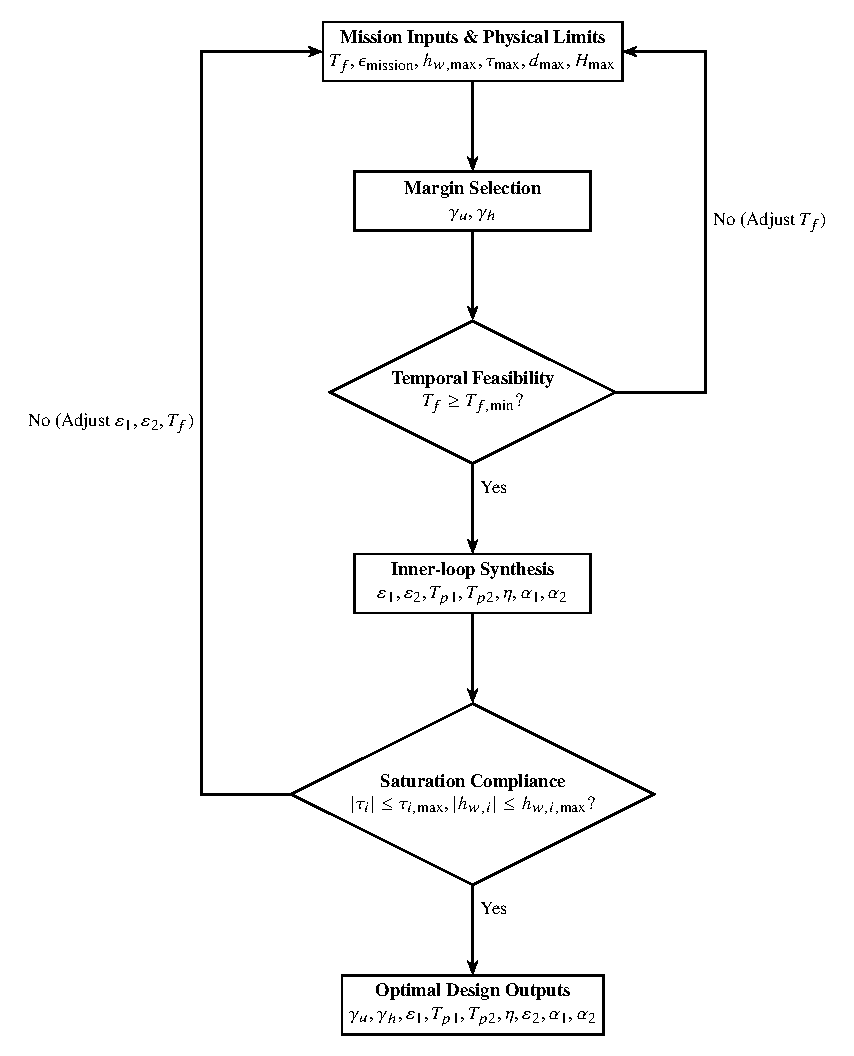
\includegraphics[height=0.5\textheight]{fig/overall.pdf}
    \caption{Parameter-synthesis methodology.}
    \label{fig:overall_design}
\end{figure}

\begin{remark}
\label{rem:balanced_synthesis}
To avoid unbalanced gains, enforce $\alpha_1=\alpha_2=\kappa\,\alpha$ with $\kappa>1$ by solving $\alpha_{1,\min}=\alpha_{2,\min}$ in \eqref{eq:alpha_min_short}.
This yields
\begin{equation}
\varepsilon_2
=\left(\frac{2T_{d,\max}\,T_{p2}}{T_{p1} \lambda_{\min}(\boldsymbol{J}_0)^{1 - \frac{\eta}{2}}}\right)^{\frac{1}{2-\eta}}
\varepsilon_1^{\frac{1-\eta}{2-\eta}}
,
\quad
\alpha=\frac{\delta_1\,\eta\,T_{p1}}{\pi}\left(\frac{\sqrt{2}}{\varepsilon_1}\right)^{1-\eta}
\end{equation}
followed by $\alpha_1=\alpha_2=\kappa\,\alpha$. This provides a unique parameter set from mission inputs.
\end{remark}


% =========================
% Section 4 (before Case 1): concise intro + unified setup table + planning paragraph
% =========================

\section{Simulation Results}
\label{section:simulation}

This section presents simulation results to validate the effectiveness of the proposed EPTPAC framework.
Table~\ref{tab:sim_setup_all} summarizes the spacecraft parameters, actuator limits, and boundary conditions.
The simulation horizon extends to $T_{\mathrm{sim}}>T_f$, with the reference held at the target for $t\ge T_f$.

\begin{table}[ht]
\centering
\caption{Common simulation settings and boundary conditions}
\label{tab:sim_setup_all}
\begin{tabular}{@{}l l@{}}
\toprule
\textbf{Symbol} & \textbf{Value} \\
\midrule
$\boldsymbol{J}_0$ &
$\mathrm{diag}([200,\ 250,\ 300])~\si{kg\cdot m^2}$ \\
$\Delta\boldsymbol{J}$ &
$5\% \boldsymbol{J}_0 $ \\
$\tau_{i,\max}$ &
$\SI{0.2}{N\cdot m}$ \\
$h_{w,i,\max}$ &
$\SI{4.0}{kg\cdot m^2/s}$ \\
$\boldsymbol{h}_{w,0}$ &
$[0,\ 0,\ 0]^\top~\si{kg\cdot m^2/s}$ \\
$\boldsymbol{d}(t)$ &
$0.01\,[\sin(2t),\ \cos(t),\ \cos(t+2)]^\top~\si{N\cdot m}$ \\
$T_{d,\max}$ &
$\SI{0.03}{N\cdot m}$ \\
$H_{\max}$ &
$\SI{0.1}{kg\cdot m^2/s}$ \\
$\boldsymbol{\sigma}(0)$ &
$[0.2,\ 0.3,\ -0.3]^\top$ \\
$\boldsymbol{\sigma}_{\mathrm{target}}$ &
$[0,\ 0,\ 0]^\top$ \\
$\boldsymbol{\omega}(0)$ &
$[0,\ 0,\ 0]^\top~\si{rad/s}$ \\
$\boldsymbol{\omega}_{\mathrm{target}}$ &
$[0,\ 0,\ 0]^\top~\si{rad/s}$ \\\bottomrule
\end{tabular}
\end{table}

The nominal trajectory reference $(\boldsymbol{\sigma}_d,\boldsymbol{\omega}_d)$ is generated offline by solving the constrained OCP
\eqref{eq:OCP_slack} via GPOPS-II.
Following Remarks~\ref{rem:gamma_u_selection}--\ref{rem:gamma_h_selection},
$\gamma_u=0.2$ and $\gamma_h=0.1$ are adopted.
The minimum feasible terminal time is $T_{f,\min}\approx\SI{95}{s}$ via Appendix~\ref{app:bangbang};
all cases use $T_f\ge\SI{110}{s}$ to ensure feasibility.

Three cases are conducted to validate different aspects of the framework.
Case~1 verifies fundamental tracking performance under dual saturation.
Case~2 assesses prescribed-time convergence and accuracy tunability.
Case~3 benchmarks the proposed framework against the torque-saturated prescribed-time controller of~\cite{xu_distributed_2022} (hereafter Ref.~\cite{xu_distributed_2022}) under torque-only and dual-saturation conditions.

\subsection{Case 1: Nominal Performance Validation}
The mission parameters are as follows: terminal time $T_f=\SI{120}{s}$, mission accuracy $\varepsilon_1=10^{-5}$, 
prescribed-time exponent $\eta=0.2$, and time allocations $T_{p2}=\SI{15}{s}$, $T_{p1}=\SI{100}{s}$.
Following the synthesis methodology in Section~\ref{overall_design} with $\kappa=1.2$, the inner-loop parameters are determined to be $\varepsilon_2=6.43\times10^{-5}$ and $\alpha_1=\alpha_2=6.34$.
The practical convergence bounds $\varepsilon_{\delta_1}=7.96\times10^{-6}$ and $\varepsilon_{\delta_2}=5.13\times10^{-5}$ 
satisfy $\varepsilon_{\delta_i}<\varepsilon_i$.

Fig.~\ref{fig:tracking_performance} shows that the spacecraft attitude and angular velocity closely track the reference trajectory, which reaches the target state at $t = T_f$.
As shown in Figs.~\ref{fig:convergence_behavior} and~\ref{fig:constraint_satisfaction}, all tracking errors remain within the prescribed-accuracy sets and both control torques and wheel momentum stay within their respective limits over $[0, T_f]$.

\begin{figure}[ht]
    \centering
    \begin{minipage}[b]{0.48\linewidth}\centering
        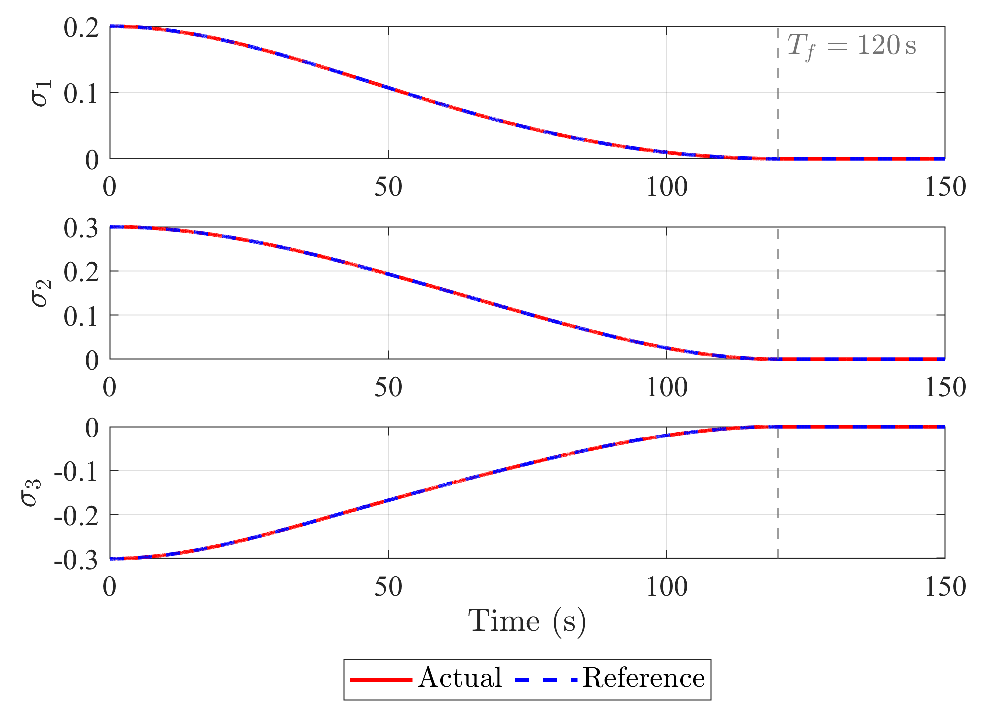
\includegraphics[width=\linewidth]{fig/Case1_Results_AttitudeComparison_tf120.0.pdf}\\[2pt]
        \footnotesize (a) Attitude MRPs
    \end{minipage}\hfill
    \begin{minipage}[b]{0.48\linewidth}\centering
        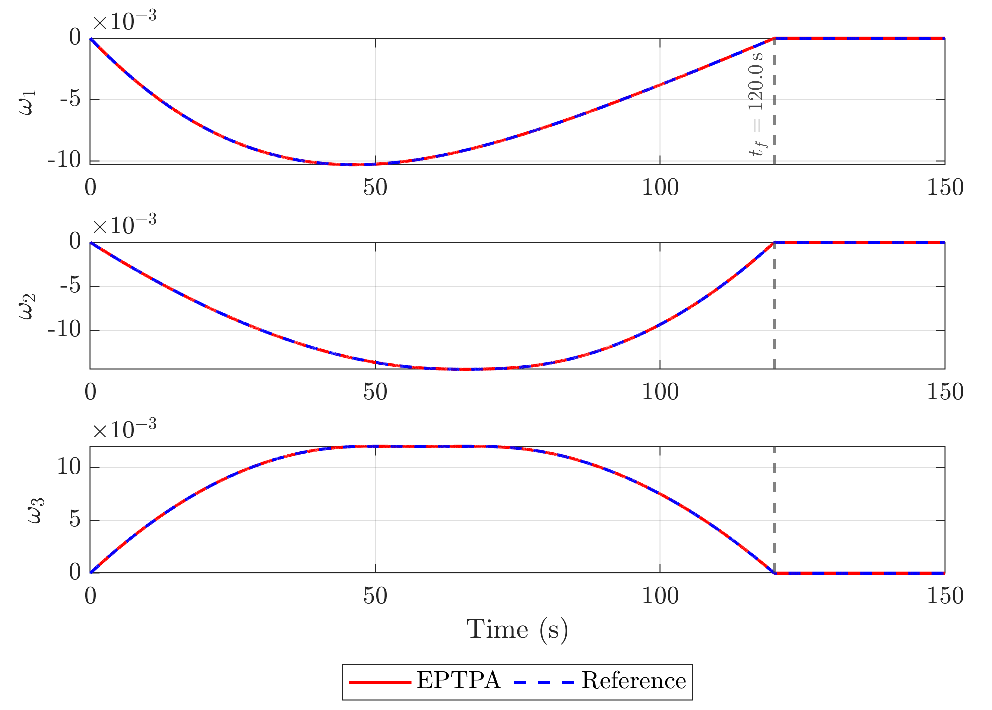
\includegraphics[width=\linewidth]{fig/Case1_Results_omega_AttitudeComparison_tf120.0.pdf}\\[2pt]
        \footnotesize (b) Angular velocity
    \end{minipage}
    \caption{Case~1: Reference tracking in MRPs and angular rates.}
    \label{fig:tracking_performance}
\end{figure}

\begin{figure}[ht]
    \centering
    \begin{minipage}[b]{0.32\linewidth}\centering
        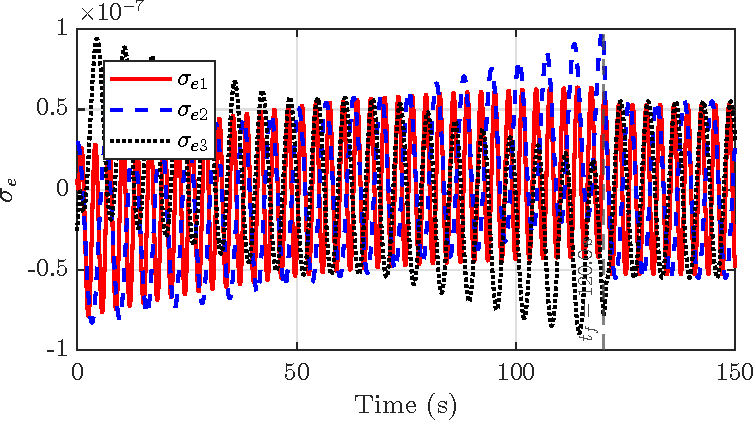
\includegraphics[width=\linewidth]{fig/Case1_Results_AttitudeError_tf120.0.pdf}\\[2pt]
        \footnotesize (a) $ \boldsymbol{\sigma}_e $
    \end{minipage}\hfill
    \begin{minipage}[b]{0.32\linewidth}\centering
        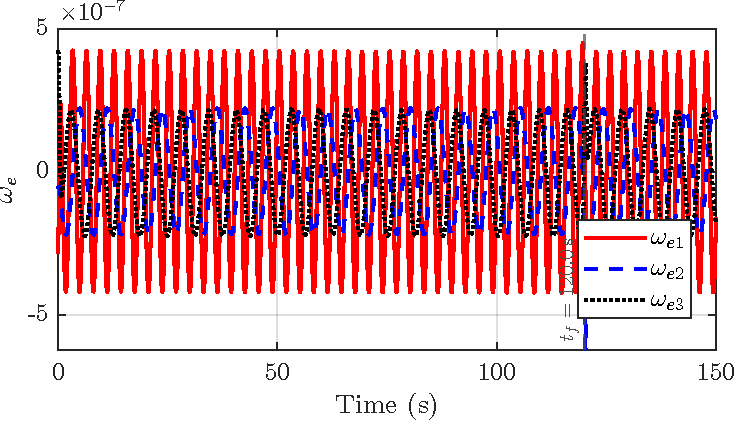
\includegraphics[width=\linewidth]{fig/Case1_Results_AngularRateError_tf120.0.pdf}\\[2pt]
        \footnotesize (b) $ \boldsymbol{\omega}_e $
    \end{minipage}\hfill
    \begin{minipage}[b]{0.32\linewidth}\centering
        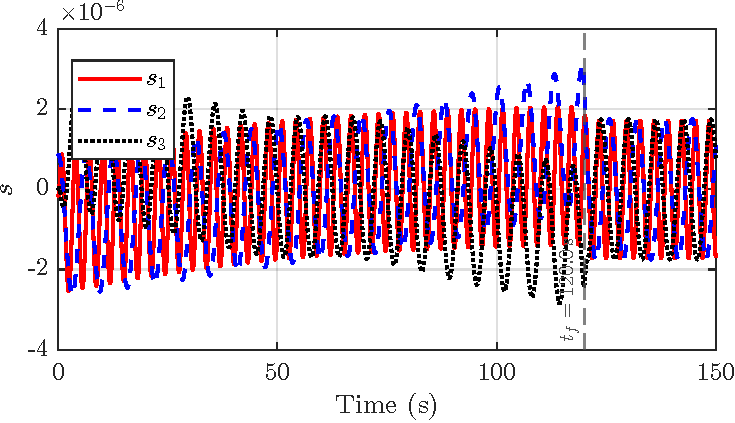
\includegraphics[width=\linewidth]{fig/Case1_Results_sError_tf120.0.pdf}\\[2pt]
        \footnotesize (c) $ \boldsymbol{s} $
    \end{minipage}
    \caption{Case~1: Error responses}
    \label{fig:convergence_behavior}
\end{figure}

\begin{figure}[ht]
    \centering
    \begin{minipage}[b]{0.48\linewidth}\centering
        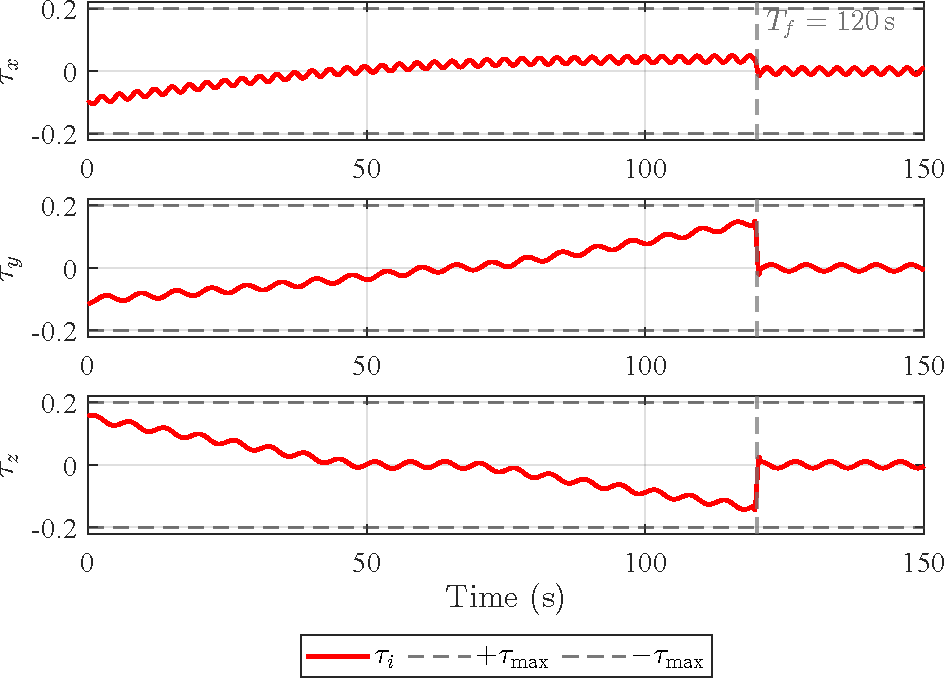
\includegraphics[width=\linewidth]{fig/Case1_Results_ControlTorque_tf120.0.pdf}\\[2pt]
        \footnotesize (a) $ \boldsymbol{\tau} $
    \end{minipage}\hfill
    \begin{minipage}[b]{0.48\linewidth}\centering
        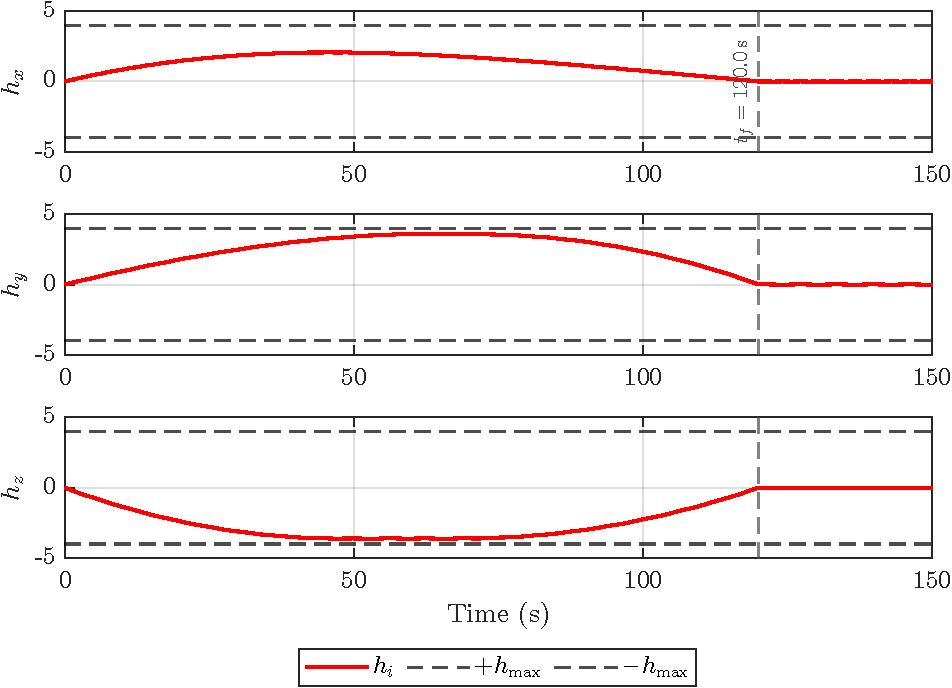
\includegraphics[width=\linewidth]{fig/Case1_Results_WheelMomentum_tf120.0.pdf}\\[2pt]
        \footnotesize (b) $ \boldsymbol{h}_w $
    \end{minipage}
    \caption{Case~1: Torque and wheel momentum.}
    \label{fig:constraint_satisfaction}
\end{figure}

In summary, Case~1 validates the baseline performance of the EPTPAC framework under dual saturation.

\subsection{Case 2: Prescribed Performance Assessment}
\label{sec:case2_prescribed_perf}

This case evaluates the two defining characteristics of the EPTPAC framework, exact terminal-time convergence
and prescribed-accuracy tunability, in a unified assessment.

\subsubsection{Time-flexibility.}
The terminal time is swept over $T_f\in\{110,\,120,\,130,\,140\}~\si{s}$, with $\varepsilon_1=10^{-5}$, $\eta=0.2$, $T_{p2}=\SI{15}{s}$, and $T_{p1}=T_f-\SI{20}{s}$.
For each $T_f$, the OCP generates a constraint-feasible reference trajectory, and
the inner-loop parameters are synthesized via the balanced rule with $\kappa=1.2$
following the procedure in Section~\ref{overall_design}.

Fig.~\ref{fig:Case2_qe_xyz} shows that the target-pointing error converges at the respective terminal times for all tested values, with the attitude error entering the prescribed accuracy only $0.24$--$0.25~\si{s}$ prior to $T_f$ (relative timing error below $0.06\%$).

\begin{figure}[ht]
  \centering
  \begin{minipage}[b]{0.32\linewidth}\centering
    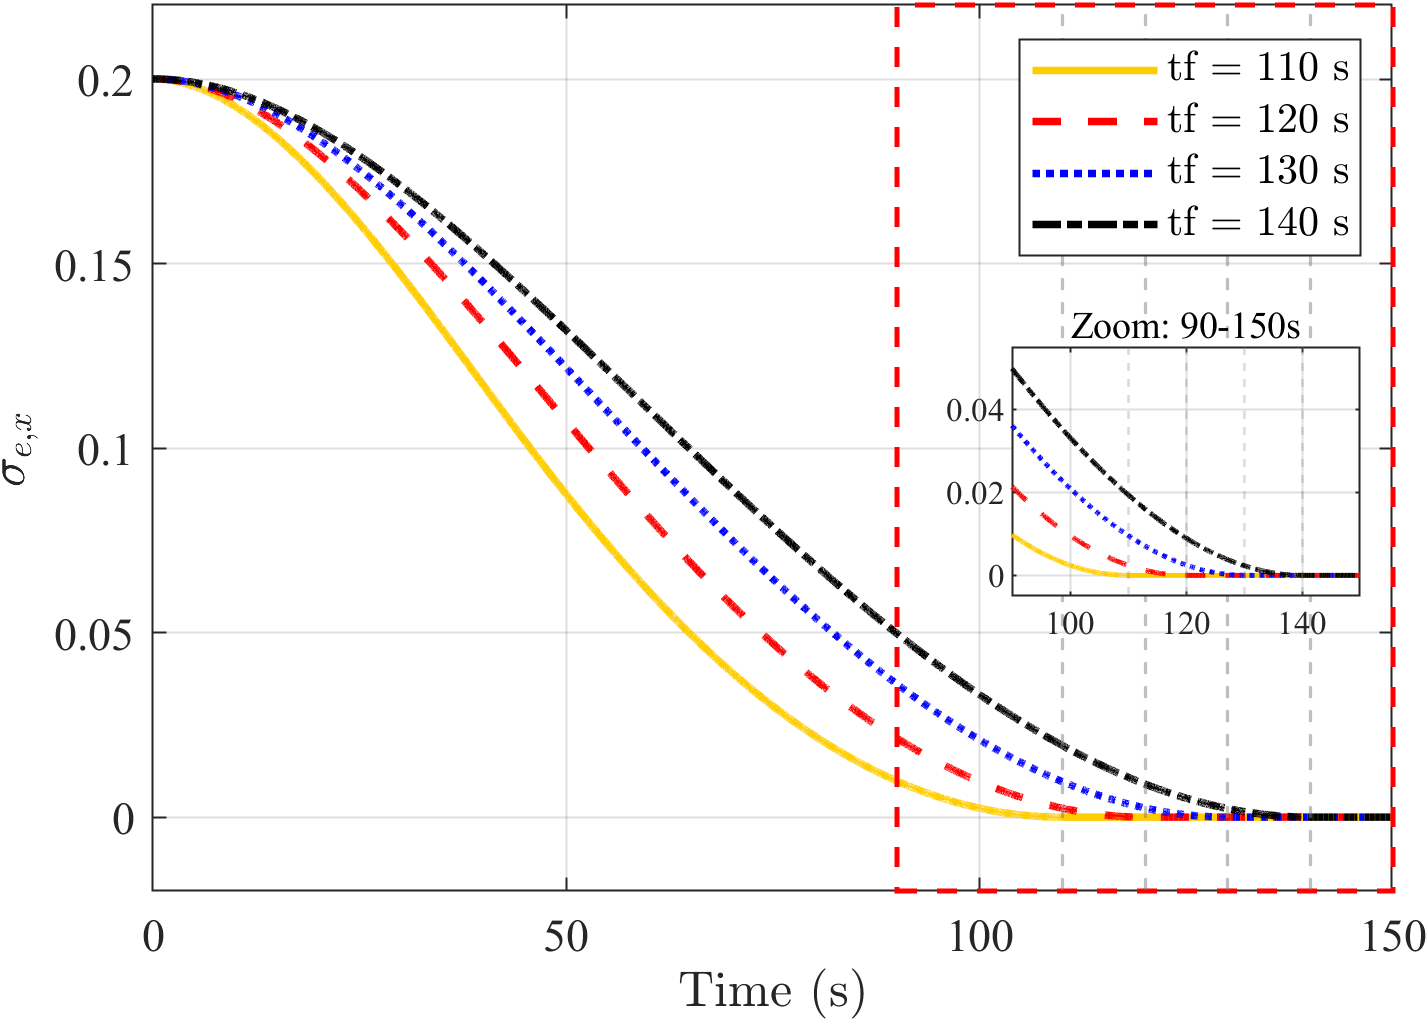
\includegraphics[width=\linewidth]{fig/qe_x_comparison.png}\\[2pt]
    \footnotesize (a) $ \sigma_{e1, \mathrm{tar}} $
  \end{minipage}\hfill
  \begin{minipage}[b]{0.32\linewidth}\centering
    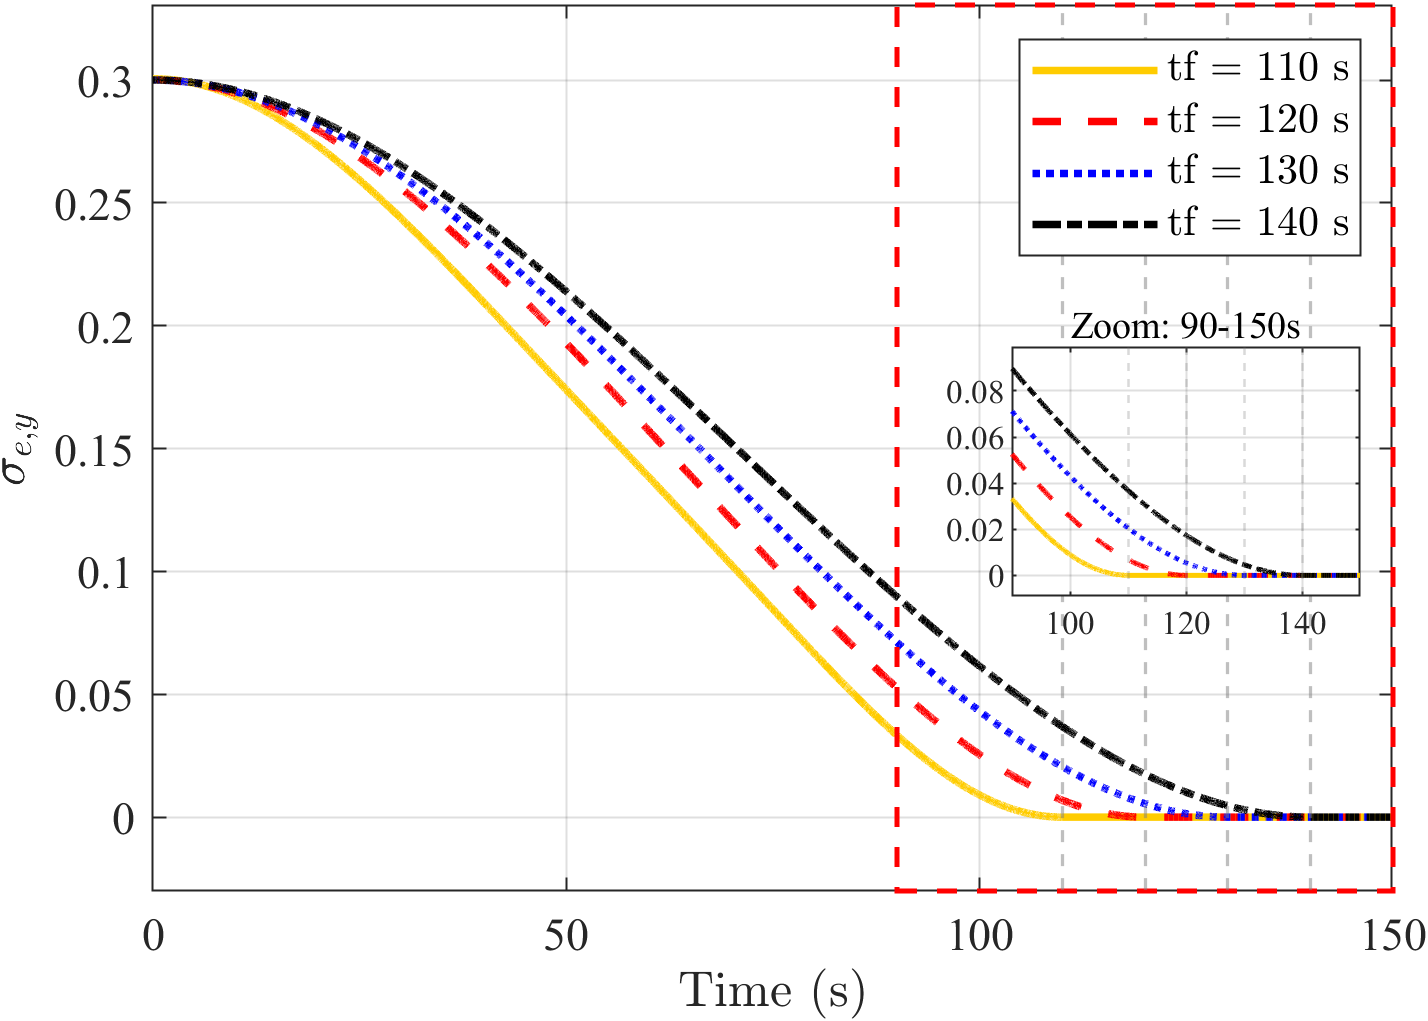
\includegraphics[width=\linewidth]{fig/qe_y_comparison.png}\\[2pt]
    \footnotesize (b) $ \sigma_{e2, \mathrm{tar}} $
  \end{minipage}\hfill
  \begin{minipage}[b]{0.32\linewidth}\centering
    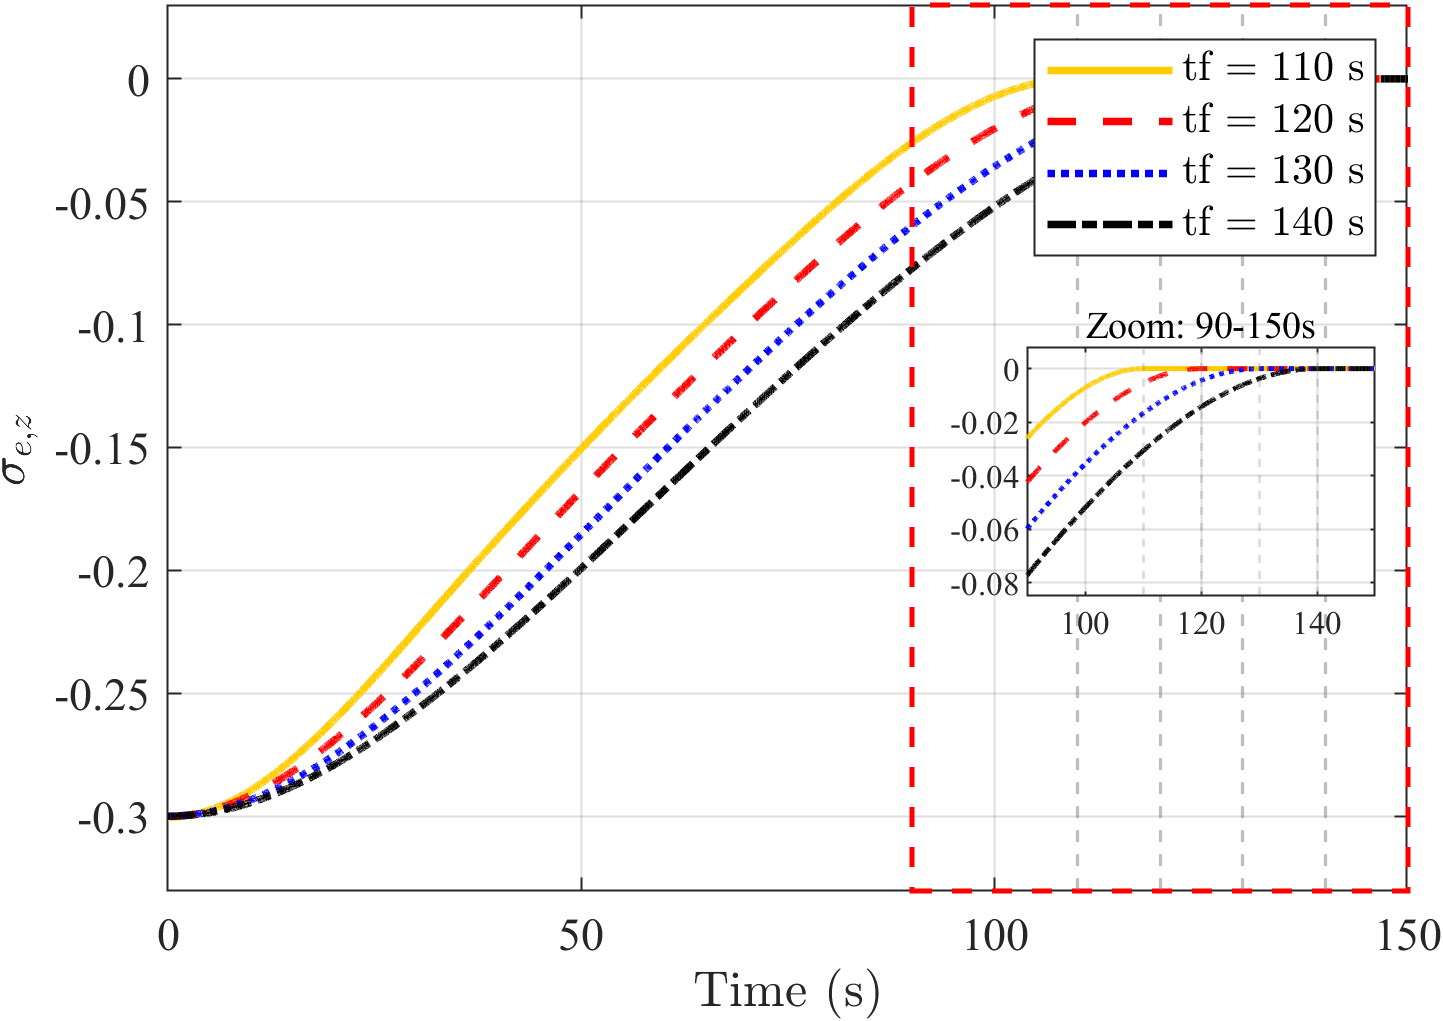
\includegraphics[width=\linewidth]{fig/qe_z_comparison.png}\\[2pt]
    \footnotesize (c) $ \sigma_{e3, \mathrm{tar}} $
  \end{minipage}
  \caption{Case~2: MRP error components for different $T_f$}
  \label{fig:Case2_qe_xyz}
\end{figure}

\subsubsection{Accuracy-sweep.}
To evaluate accuracy tunability, the prescribed accuracy is swept over $\varepsilon_1\in\{10^{-4},\,10^{-5},\,10^{-6},\,10^{-7}\}$ with $T_f=\SI{120}{s}$ fixed.
For each $\varepsilon_1$, the inner-loop parameters are synthesized via the balanced rule with $\kappa=1.2$
following Section~\ref{overall_design}.

As shown in Fig.~\ref{fig:case3_precision_compare}, all four settings achieve their prescribed accuracies within $T_f$.
Higher precision requires higher gains: tightening $\varepsilon_1$ from $10^{-4}$ to $10^{-7}$
increases $\alpha_1=\alpha_2$ from $4.30$ to $24.78$.

\begin{figure}[ht]
    \centering
    \begin{minipage}[b]{0.48\linewidth}\centering
        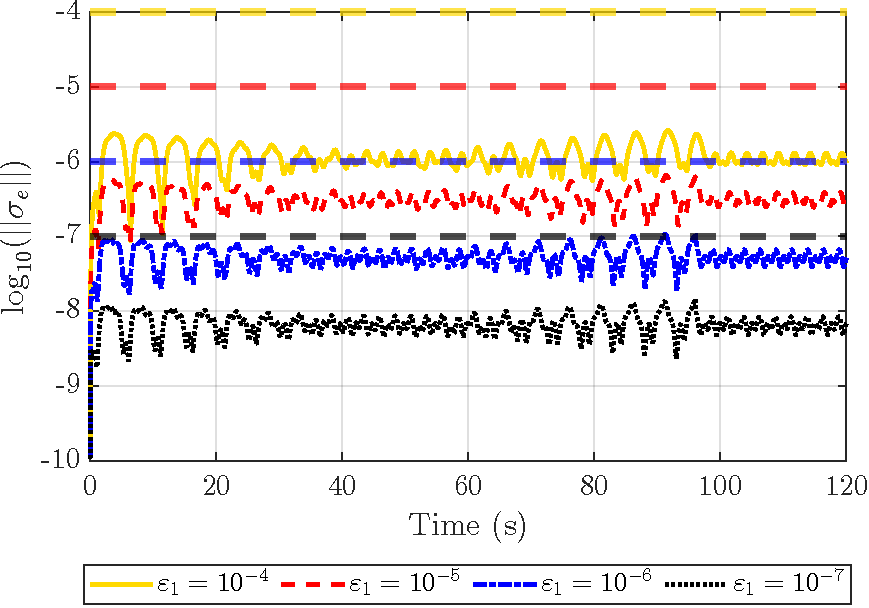
\includegraphics[width=\linewidth]{fig/CaseSweep_MRPErrorNorm_log10.pdf}\\[2pt]
        \footnotesize (a) $\log_{10}(\|\boldsymbol{\sigma}_e\|)$ with $\varepsilon_1$ thresholds
    \end{minipage}\hfill
    \begin{minipage}[b]{0.48\linewidth}\centering
        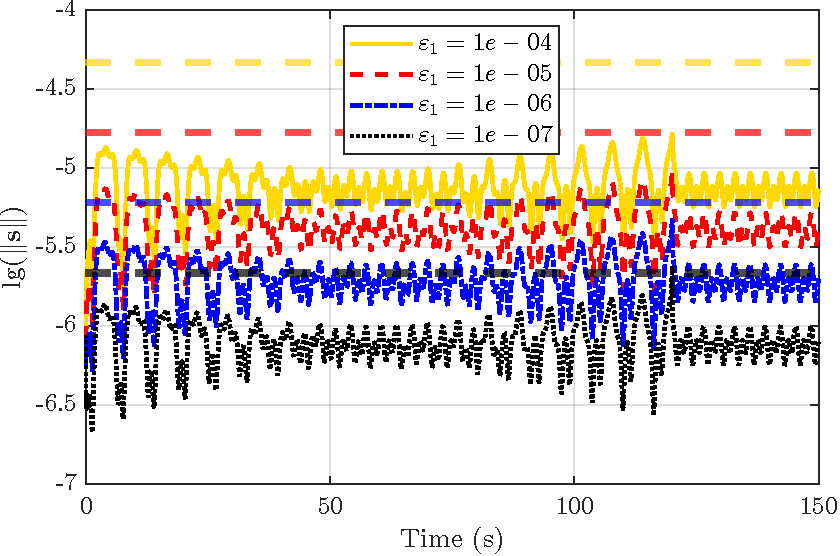
\includegraphics[width=\linewidth]{fig/CaseSweep_SlidingNorm_log10.pdf}\\[2pt]
        \footnotesize (b) $\log_{10}(\|\boldsymbol{s}\|)$ with $\varepsilon_2$ thresholds
    \end{minipage}
    \caption{Case~2: Log-scale comparison of $\|\boldsymbol{\sigma}_e\|$ and $\|\boldsymbol{s}\|$ for different $\varepsilon_1$}
    \label{fig:case3_precision_compare}
\end{figure}

Case~2 confirms that the EPTPAC framework simultaneously delivers exact terminal-time convergence
with sub-percent temporal precision and tunable steady-state accuracy across four orders of magnitude.

\subsection{Case 3: Comparison with Ref.~\cite{xu_distributed_2022}}

To evaluate the advantage of the proposed framework over existing methods, this case compares EPTPAC with the torque-saturated prescribed-time controller of~\cite{xu_distributed_2022}, which addresses torque limits but does not account for wheel-momentum constraints.
Two scenarios are conducted: Case~3.1 considers 
torque saturation only, thereby providing a fair comparison under identical constraint 
assumptions; Case~3.2 enforces dual saturation to assess how the 
additional momentum constraint affects controller performance.

\subsubsection{Case 3.1: Torque-only saturation}

This scenario evaluates terminal-time tracking performance under torque saturation only
($\tau_{i,\max}=0.2~\si{N\cdot m}$) with two prescribed terminal times:
$T_f=300~\si{s}$ and $T_f=150~\si{s}$.

\begin{figure}[ht]
    \centering
    \subfloat[Attitude error ($T_f=300$ s)]{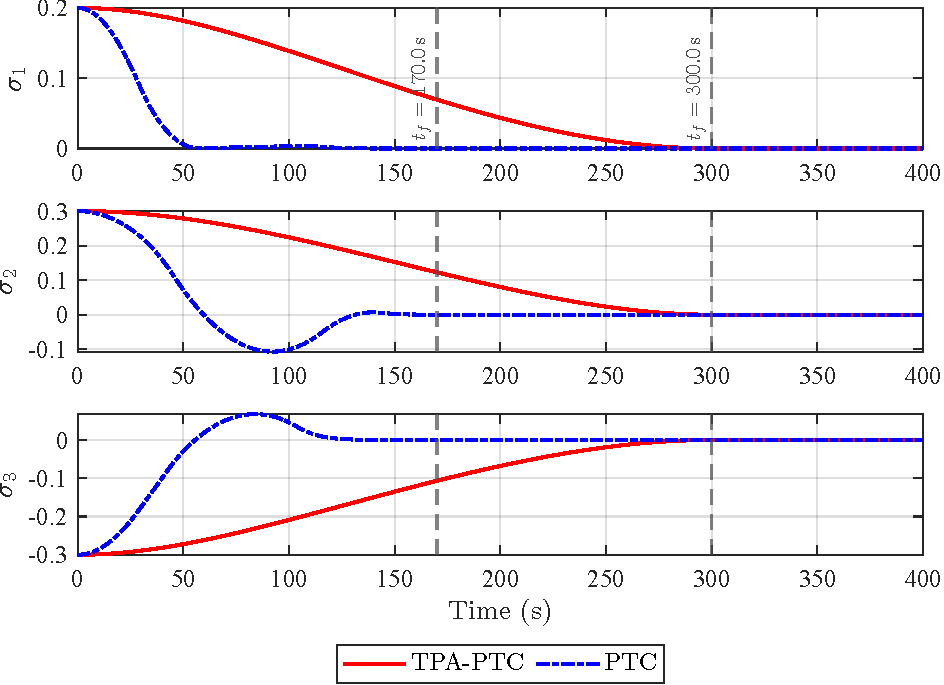
\includegraphics[width=0.48\linewidth]{fig/PTC_compare_Attitude__t_total400.0.pdf}\label{fig:err300}}
    \hfill
    \subfloat[Control torque ($T_f=300$ s)]{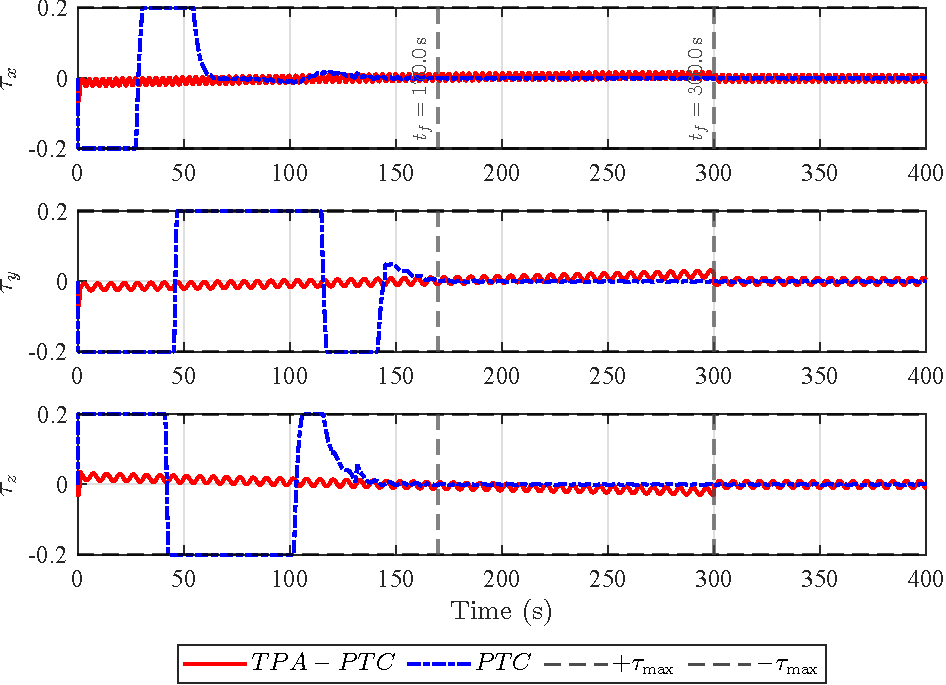
\includegraphics[width=0.48\linewidth]{fig/PTC_compare_ControlTorque_t_total400.0.pdf}\label{fig:tau300}}
    \\
    \subfloat[Attitude error ($T_f=150$ s)]{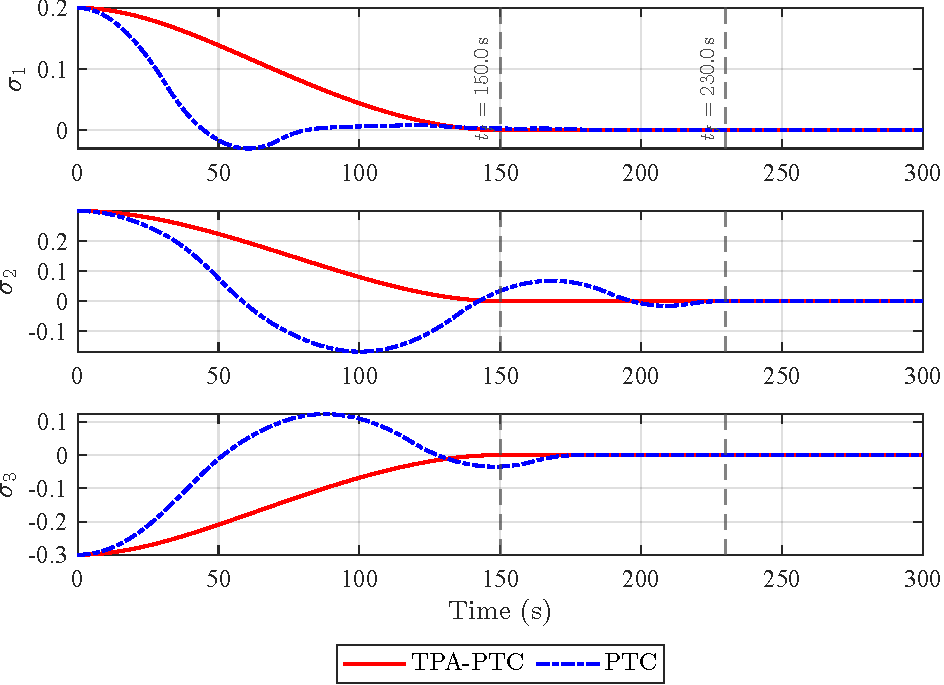
\includegraphics[width=0.48\linewidth]{fig/PTC_compare_Attitude__t_total300.0.pdf}\label{fig:err150}}
    \hfill
    \subfloat[Control torque ($T_f=150$ s)]{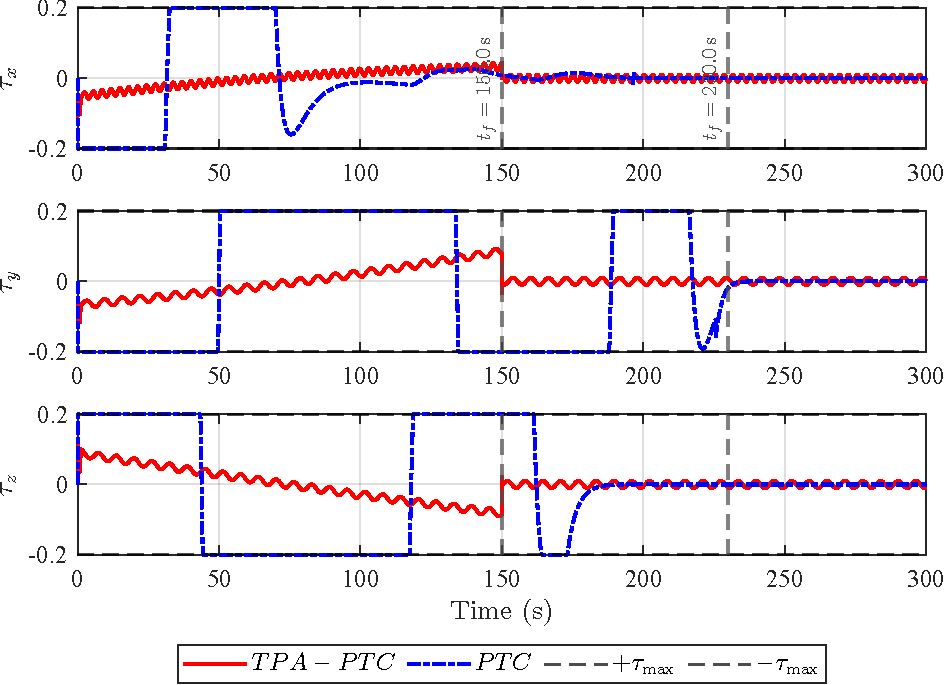
\includegraphics[width=0.48\linewidth]{fig/PTC_compare_ControlTorque_t_total300.0.pdf}\label{fig:tau150}}
    \caption{Case 3.1: Performance comparison under torque-only saturation}
    \label{fig:case4_1_comparison}
\end{figure}

For the $T_f=300~\si{s}$ case, as depicted in Figs.~\ref{fig:err300} and~\ref{fig:tau300},
Ref.~\cite{xu_distributed_2022} exhibits pronounced conservatism, converging around $150~\si{s}$---only 50\% of the prescribed duration.
Such premature convergence necessitates unnecessarily aggressive control action in the early stage,
leading to excessive torque expenditure.

A more critical breakdown is observed when $T_f$ is reduced to $150~\si{s}$,
approaching the minimum feasible maneuver time $T_{f,\min}$ (Appendix~\ref{app:bangbang}).
As shown in Figs.~\ref{fig:err150} and~\ref{fig:tau150},
Ref.~\cite{xu_distributed_2022} loses prescribed-time convergence entirely,
with the response delayed until approximately $230~\si{s}$.
This failure occurs because the high-gain feedback mechanism does not account for
physical feasibility under tight actuator constraints.
The resulting torque saturation compromises the nominal stability guarantees of the prescribed-time control law.

In contrast, EPTPAC consistently achieves exact convergence at both prescribed terminal times
with smooth, feasible control profiles. These results underscore that physical realizability
is a fundamental requirement for reliable terminal-time tracking.

\subsubsection{Case 3.2: Dual saturation}

This scenario examines controller performance under dual-saturation constraints with $T_f=300~\si{s}$.

\begin{figure}[ht]
    \centering
    \subfloat[Attitude error]{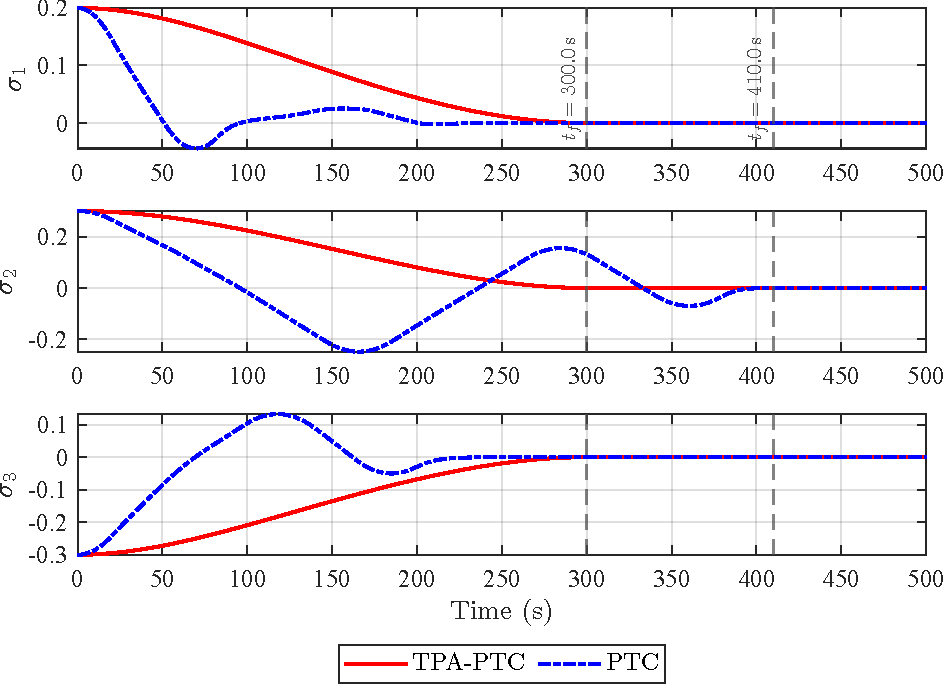
\includegraphics[width=0.48\linewidth]{fig/PTC_compare_Attitude__t_total500.0.pdf}\label{fig:err_dual}}
    \hfill
    \subfloat[Angular velocity error]{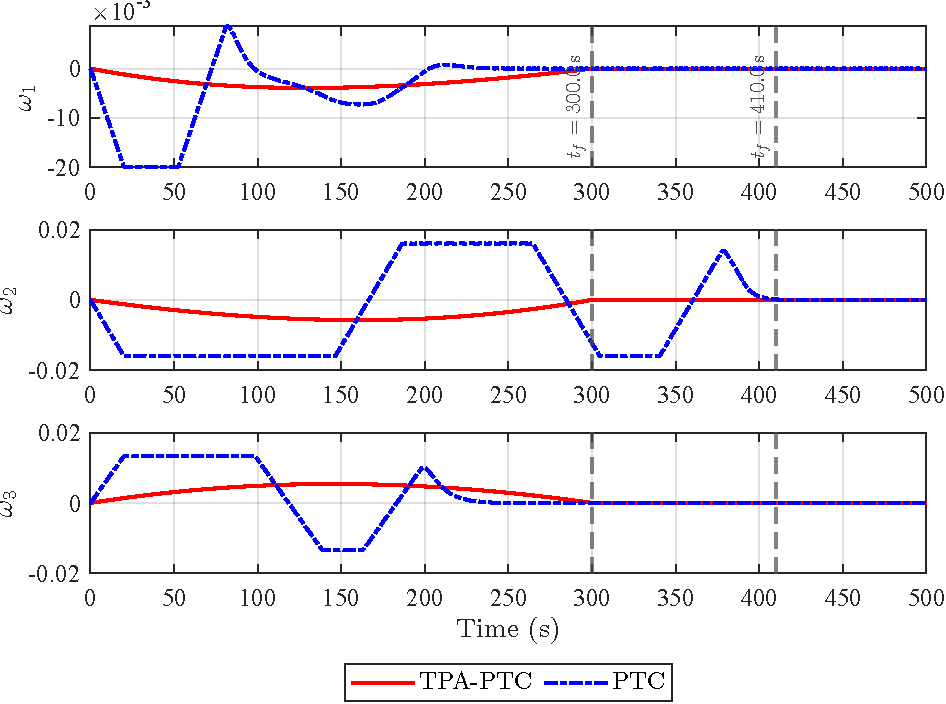
\includegraphics[width=0.48\linewidth]{fig/PTC_compare_omega__t_total500.0.pdf}\label{fig:omega_dual}}
    \\
    \subfloat[Control torque]{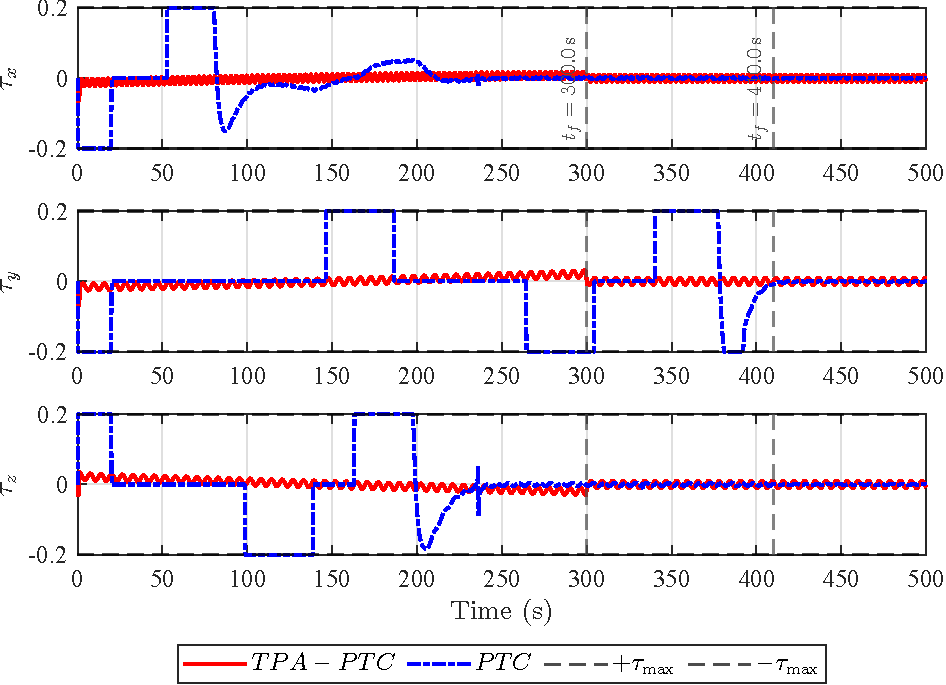
\includegraphics[width=0.48\linewidth]{fig/PTC_compare_ControlTorque_t_total500.0.pdf}\label{fig:tau_dual}}
    \hfill
    \subfloat[Wheel momentum]{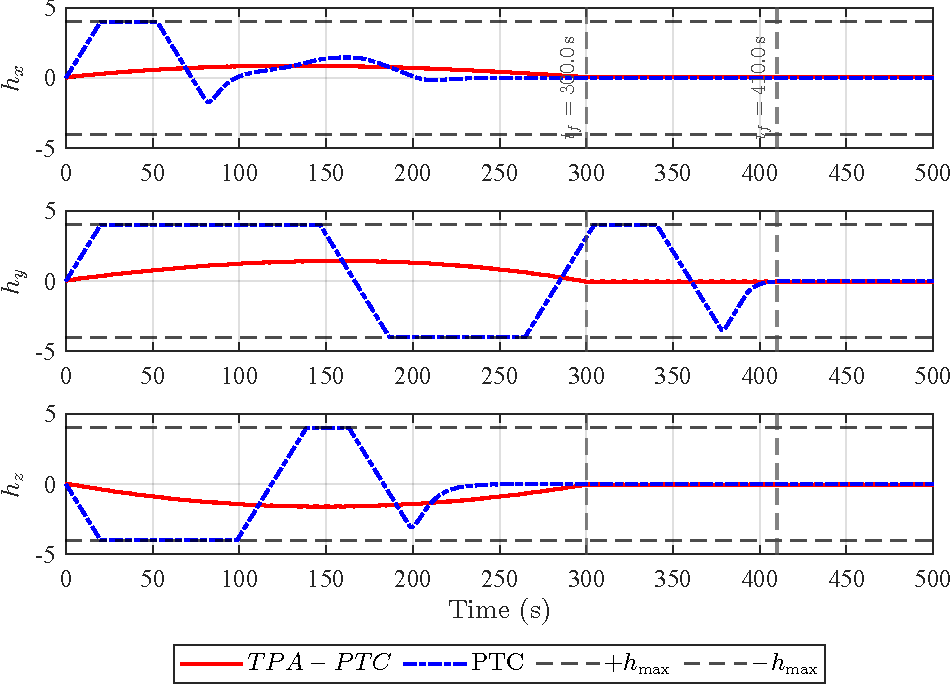
\includegraphics[width=0.48\linewidth]{fig/PTC_compare_WheelMomentum_t_total500.0.pdf}\label{fig:hw_dual}}

    \caption{Case 3.2: Performance comparison under dual saturation}
    \label{fig:case4_2_comparison}
\end{figure}

As shown in Fig.~\ref{fig:case4_2_comparison}, Ref.~\cite{xu_distributed_2022}
neglects momentum constraints and commands impulsive torques,
leading to rapid momentum accumulation that drives the reaction wheels into saturation
(Figs.~\ref{fig:tau_dual} and~\ref{fig:hw_dual}).
Once saturated, the spacecraft suffers a complete loss of control authority and enters an uncontrolled drift phase,
with convergence severely delayed to $410~\si{s}$---far exceeding the prescribed $300~\si{s}$.
In contrast, EPTPAC modulates the torque profile to prevent momentum saturation,
achieving exact convergence at $t=300~\si{s}$.

In summary, Case~3 underscores the necessity of physical realizability in prescribed-time control.
Case~3.1 shows that existing PTC methods exhibit either excessive conservatism or loss of convergence guarantees
when $T_f$ approaches $T_{f,\min}$.
Case~3.2 reveals that unmanaged momentum accumulation exacerbates these limitations,
leading to prolonged loss of control authority.
The EPTPAC framework circumvents both issues through constraint-aware co-design
of the planning and control layers.

\section{Conclusion}
\label{section:conclusion}
This note proposed a two-loop EPTPAC framework for spacecraft actuated by reaction wheels to achieve prescribed accuracy at a user-specified terminal time under dual saturation.
The outer loop employs a constrained optimal control problem to generate a reference trajectory that respects dual-saturation constraints, while the inner loop uses a robust prescribed-time prescribed-accuracy controller to track the reference within the desired accuracy by the terminal time.
Through this decoupled architecture, the proposed framework effectively overcomes the fundamental shortcomings of existing PTC methods, namely the inherent conservatism and insufficient consideration of dual saturation. Furthermore, by identifying the minimum feasible maneuver time $T_{f,\min}$ and establishing a parameter-synthesis methodology, the proposed framework significantly strengthens engineering realizability while streamlining the design process.
Numerical simulations validated the effectiveness of the proposed framework in achieving exact terminal-time convergence, tunable precision, and dual-saturation compliance.
Future work will focus on multi-spacecraft cooperative maneuvers.

\appendix
\section{Estimate of Minimum Feasible Maneuver Time}
\label{app:bangbang}

This appendix provides a practical estimate of $T_{f,\min}$ for use in Assumption~\ref{ass:feasible_Tf}.
Given initial attitude $\boldsymbol{\sigma}_e(0)$, the principal rotation angle $\theta$ and axis $\boldsymbol{e}$ satisfy
$\theta = 4\arctan(\|\boldsymbol{\sigma}_e(0)\|)$ and
$\boldsymbol{e} = \boldsymbol{\sigma}_e(0)/\|\boldsymbol{\sigma}_e(0)\|$ (or any unit vector if $\boldsymbol{\sigma}_e(0)=\boldsymbol{0}$).
Define $J_e = \boldsymbol{e}^\top\boldsymbol{J}_0\boldsymbol{e}$.
Under component-wise torque limits $|\tau_i|\le\tau_{i,\max}$, the maximum torque projection along $\boldsymbol{e}$ is
$\tau_{e,\max}= \sum_{i=1}^{3}|e_i|\tau_{i,\max}$.

Assuming $\boldsymbol{h}_w(0)=\boldsymbol{0}$ and a bang-bang allocation $\tau_i=\mathrm{sgn}(e_i)\tau_{i,\max}$,
the maximum duration before momentum saturation is
$t_h = \min_i h_{w,i,\max}/\tau_{i,\max}$.
For a rest-to-rest rotation about $\boldsymbol{e}$,
the peak rate is $\omega_{\max}= \tau_{e,\max}t_h/J_e$
and the no-coast angle is $\theta_h = \tau_{e,\max}t_h^2/J_e$.
The minimum-time estimate is then
\begin{equation}
T_{f,\min}\approx
\begin{cases}
2\sqrt{J_e\theta/\tau_{e,\max}}, & \theta \le \theta_h,\\[6pt]
2t_h + (\theta-\theta_h)/\omega_{\max}, & \theta > \theta_h
\end{cases}
\label{eq:app_Tmin_piecewise}
\end{equation}

\newpage

\section*{Acknowledgments}

This work was supported in part by the National Key Research and Development Program of China under Grant Nos. 2021YFC2202901, 2023YFC2206004, and 2024YFC2207203; the National Natural Science Foundation of China under Grant No. U25B2052; the Excellent Youth Fund of the Heilongjiang Provincial Natural Science Foundation under Grant No. YQ2024F010; and the Fund of the State Key Laboratory of Micro-Spacecraft Rapid Design and Intelligent Cluster under Grant No. MS02240103.

During the preparation of this work, the authors used an AI-assisted writing tool for language polishing. All scientific content, methodology, and conclusions are entirely the work of the authors.

\bibliography{sample}


\end{document}
